
% Safely inserts your illustration full-bleed on its own page.
% This completely bypasses the page builder, headers, and geometry bugs!
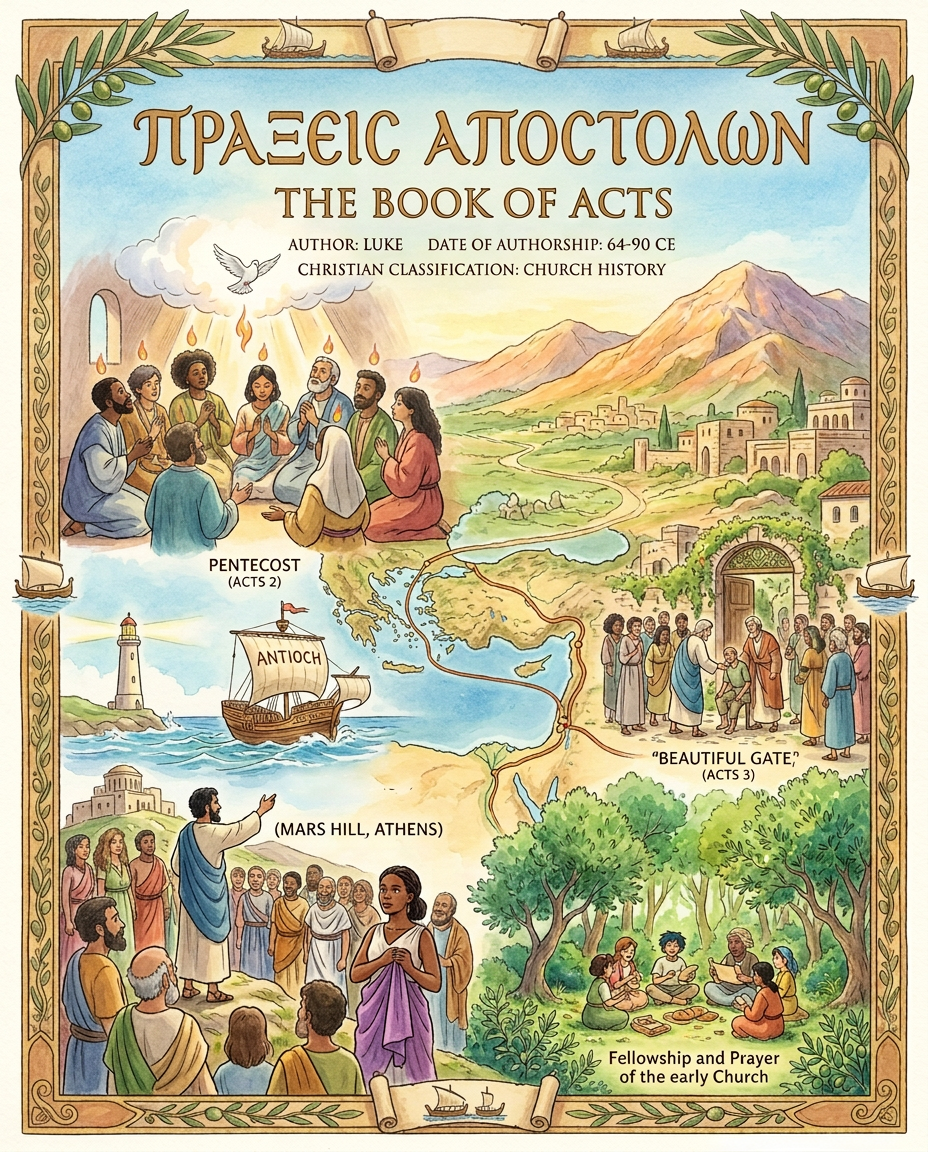
\includepdf[pages=1, fitpaper=false, width=\paperwidth, height=\paperheight, , keepaspectratio=false]{images/divider2/acts2.png}
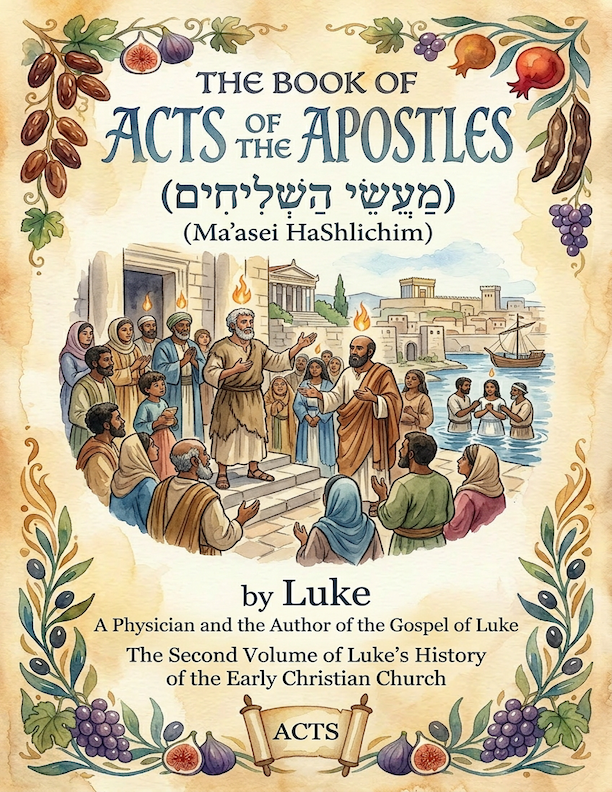
\includepdf[pages=1, fitpaper=false, width=\paperwidth, height=\paperheight, , keepaspectratio=false]{images/divider1/acts.png}

\includepdf[pages=1, fitpaper=false, width=\paperwidth, height=\paperheight, , keepaspectratio=false]{images/8.5x11-Dot-Grid.png}

\includepdf[pages=1, fitpaper=false, width=\paperwidth, height=\paperheight, , keepaspectratio=false]{images/8.5x11-Dot-Grid.png}

\mybook{The Acts of the Emissaries}
\vspace{-1.36in}

\mychapter{} \myverse*{}The first book I wrote, Theophilus, concerned all that Yeshua began
both to do and to teach,
\myverse{}until the day in which he was received up, after he had given commandment through
the Holy Spirit to the emissaries whom he had chosen.
\myverse{}To these he also showed himself alive after he suffered, by many proofs, appearing
to them over a period of forty days and speaking about God’s Kingdom.
\myverse{}Being assembled together with them, he commanded them,
\textcolor{crimson}{“Don’t depart from Jerusalem, but wait for the promise of the Father, which you heard from me.
}
\myverse{}\textcolor{crimson}{For Yochanan indeed immersed in water, but you will be immersed in the Holy
	Spirit not many days from now.”}

\myverse{}Therefore, when they had come together, they asked him, “Lord,
are you now restoring the kingdom to Israel?”

\myverse{}He said to them,
\textcolor{crimson}{“It isn’t for you to know times or seasons which the Father has set within his own authority.
}
\myverse{}\textcolor{crimson}{But you will receive power when the Holy Spirit has come upon you. You will
	be witnesses to me in Jerusalem, in all Judea and Samaria, and to the uttermost parts of the earth.”}

\myverse{}When he had said these things, as they were looking, he was taken
up, and a cloud received him out of their sight.
\myverse{}While they were looking steadfastly into the sky as he went, behold,\footnote{1:10 “Behold”, from “ἰδοὺ”, means look at, take notice, observe, see, or gaze at. It is often used
	as an interjection.} two men stood by them in white clothing,
\myverse{}who also said, “You men of Galilee, why do you stand looking into the sky?
This Yeshua, who was received up from you into the sky, will come back in the same way as you saw him
going into the sky.”

\myverse{}Then they returned to Jerusalem from the mountain called Olivet,
which is near Jerusalem, a Sabbath day’s journey away.
\myverse{}When they had come in, they went up into the upper room where they were staying,
that is Peter, Yochanan, Jacob, Andrew, Philip, Thomas, Bartholomew, Matthew, Jacob the son of Halfai,
Simon the Zealot, and Judah the son of Jacob.
\myverse{}All these with one accord continued steadfastly in prayer and supplication,
along with the women and Miriam the mother of Yeshua, and with his brothers.

\myverse{}In these days, Peter stood up in the middle of the disciples
(and the number of names was about one hundred twenty), and said,
\myverse{}“Brothers, it was necessary that this Scripture should be fulfilled, which
the Holy Spirit spoke before by the mouth of David concerning Judah, who was guide to those who took Yeshua.
\myverse{}For he was counted with us, and received his portion in this ministry.
\myverse{}Now this man obtained a field with the reward for his wickedness; and falling
headlong, his body burst open and all his intestines gushed out.
\myverse{}It became known to everyone who lived in Jerusalem that in their language
that field was called ‘Hakel-Dema,’ that is, ‘The field of blood.’
\myverse{}For it is written in the scroll of Psalms,

‘Let his habitation be made desolate.

Let no one dwell in it;’\footnote{1:20 Psalms 69:25}

and,

‘Let another take his office.’\footnote{1:20 Psalms 109:8}

\myverse{}“Of the men therefore who have accompanied us all the time that
the Lord Yeshua went in and out among us,
\myverse{}beginning from the immersion of Yochanan to the day that he was received up
from us, of these one must become a witness with us of his resurrection.”

\myverse{}They put forward two: Joseph called Barsabbas, who was also called
Justus, and Matthiah.
\myverse{}They prayed and said, “You, Lord, who know the hearts of all men, show which
one of these two you have chosen
\myverse{}to take part in this ministry and office of emissary from which Judah fell
away, that he might go to his own place.”
\myverse{}They drew lots for them, and the lot fell on Matthiah; and he was counted
with the Eleven emissaries.


% ACTS 2
\mychapter{} \myverse*{}Now when the day of Shavu`ot had come, they were all with one accord
in one place.
\myverse{}Suddenly there came from the sky a sound like the rushing of a mighty wind,
and it filled all the house where they were sitting.
\myverse{}Tongues like fire appeared and were distributed to them, and one sat on each
of them.
\myverse{}They were all filled with the Holy Spirit and began to speak with other languages,
as the Spirit gave them the ability to speak.

\myverse{}Now there were dwelling in Jerusalem Jews, devout men, from every
nation under the sky.
\myverse{}When this sound was heard, the multitude came together and were bewildered,
because everyone heard them speaking in his own language.
\myverse{}They were all amazed and marveled, saying to one another, “Behold, aren’t all
these who speak Galileans?
\myverse{}How do we hear, everyone in our own native language?
\myverse{}Parthians, Medes, Elamites, and people from Mesopotamia, Judea, Cappadocia,
Pontus, Asia,
\myverse{}Phrygia, Pamphylia, Egypt, the parts of Libya around Cyrene, visitors from
Rome, both Jews and proselytes,
\myverse{}Cretans and Arabians—we hear them speaking in our languages the mighty works
of God!”
\myverse{}They were all amazed and were perplexed, saying to one another, “What does
this mean?”
\myverse{}Others, mocking, said, “They are filled with new wine.”

\myverse{}But Peter, standing up with the Eleven, lifted up his voice and
spoke out to them, “You men of Judea and all you who dwell at Jerusalem, let this be known to you, and
listen to my words.
\myverse{}For these aren’t drunken, as you suppose, seeing it is only the third hour
of the day.\footnote{2:15 about 9:00 a.m.}
\myverse{}But this is what has been spoken through the prophet Joel:

\myverse{}‘It will be in the last days, says God,

that I will pour out my Spirit on all flesh.

Your sons and your daughters will prophesy.

Your young men will see visions.

Your old men will dream dreams.

\myverse{}Yes, and on my servants and on my handmaidens in those days,

I will pour out my Spirit, and they will prophesy.

\myverse{}I will show wonders in the sky above,

and signs on the earth beneath:

blood, and fire, and billows of smoke.

\myverse{}The sun will be turned into darkness,

and the moon into blood,

before the great and glorious day of the Lord comes.

\myverse{}It will be that whoever will call on the name of the Lord will
be saved.’\footnote{2:21 Joel 2:28-32}

\myverse{}“Men of Israel, hear these words! Yeshua of Nazareth, a man approved
by God to you by mighty works and wonders and signs which God did by him among you, even as you yourselves
know,
\myverse{}him, being delivered up by the determined counsel and foreknowledge of God,
you have taken by the hand of lawless men, crucified and killed;
\myverse{}whom God raised up, having freed him from the agony of death, because it was
not possible that he should be held by it.
\myverse{}For David says concerning him,

‘I saw the Lord always before my face,

for he is on my right hand, that I should not be moved.

\myverse{}Therefore my heart was glad, and my tongue rejoiced.

Moreover my flesh also will dwell in hope,

\myverse{}because you will not leave my soul in Sheol,\footnote{2:27 or, Hell}

neither will you allow your Holy One to see decay.

\myverse{}You made known to me the ways of life.

You will make me full of gladness with your presence.’\footnote{2:28 Psalms 16:8-11
}

\myverse{}“Brothers, I may tell you freely of the patriarch David, that
he both died and was buried, and his tomb is with us to this day.
\myverse{}Therefore, being a prophet, and knowing that God had sworn with an oath to
him that of the fruit of his body, according to the flesh, he would raise up the Messiah\footnote{2:30 “Messiah” means “Anointed One”.} to sit on his throne,
\myverse{}he foreseeing this, spoke about the resurrection of the Messiah, that his
soul wasn’t left in Sheol,\footnote{2:31 or, Hell} and his flesh didn’t see decay.
\myverse{}This Yeshua God raised up, to which we all are witnesses.
\myverse{}Being therefore exalted by the right hand of God, and having received from
the Father the promise of the Holy Spirit, he has poured out this which you now see and hear.
\myverse{}For David didn’t ascend into the heavens, but he says himself,

‘The Lord said to my Lord, “Sit by my right hand

\myverse{}until I make your enemies a footstool for your feet.” ’\footnote{2:35 Psalms 110:1
}

\myverse{}“Let all the house of Israel therefore know certainly that God
has made him both Lord and Messiah, this Yeshua whom you crucified.”

\myverse{}Now when they heard this, they were cut to the heart, and said
to Peter and the rest of the emissaries, “Brothers, what shall we do?”

\myverse{}Peter said to them, “Repent and be immersed, every one of you,
in the name of Yeshua the Messiah for the forgiveness of sins, and you will receive the gift of the Holy
Spirit.
\myverse{}For the promise is to you and to your children, and to all who are far off,
even as many as the Lord our God will call to himself.”
\myverse{}With many other words he testified and exhorted them, saying, “Save yourselves
from this crooked generation!”

\myverse{}Then those who gladly received his word were immersed. There
were added that day about three thousand souls.
\myverse{}They continued steadfastly in the emissaries’ teaching and fellowship, in
the breaking of bread, and prayer.
\myverse{}Fear came on every soul, and many wonders and signs were done through the
emissaries.
\myverse{}All who believed were together, and had all things in common.
\myverse{}They sold their possessions and goods, and distributed them to all, according
as anyone had need.
\myverse{}Day by day, continuing steadfastly with one accord in the temple, and breaking
bread at home, they took their food with gladness and singleness of heart,
\myverse{}praising God and having favor with all the people. The Lord added to the assembly
day by day those who were being saved.


% ACTS 3
\mychapter{} \myverse*{}Peter and Yochanan were going up into the temple at the hour of
prayer, the ninth hour.\footnote{3:1 3:00 p.m.}
\myverse{}A certain man who was lame from his mother’s womb was being carried, whom they
laid daily at the door of the temple which is called Yafeh\footnote{3:2 Beautiful}, to ask gifts for
the needy of those who entered into the temple.
\myverse{}Seeing Peter and Yochanan about to go into the temple, he asked to receive gifts
for the needy.
\myverse{}Peter, fastening his eyes on him, with Yochanan, said, “Look at us.”
\myverse{}He listened to them, expecting to receive something from them.
\myverse{}But Peter said, “I have no silver or gold, but what I have, that I give you.
In the name of Yeshua the Messiah of Nazareth, get up and walk!”
\myverse{}He took him by the right hand and raised him up. Immediately his feet and his
ankle bones received strength.
\myverse{}Leaping up, he stood and began to walk. He entered with them into the temple,
walking, leaping, and praising God.
\myverse{}All the people saw him walking and praising God.
\myverse{}They recognized him, that it was he who used to sit begging for gifts for
the needy at the Yafeh Gate of the temple. They were filled with wonder and amazement at what had happened
to him.
\myverse{}As the lame man who was healed held on to Peter and Yochanan, all the people
ran together to them in the porch that is called Solomon’s, greatly wondering.

\myverse{}When Peter saw it, he responded to the people, “You men of Israel,
why do you marvel at this man? Why do you fasten your eyes on us, as though by our own power or godliness
we had made him walk?
\myverse{}The God of Abraham, Isaac, and Jacob, the God of our fathers, has glorified
his Servant Yeshua, whom you delivered up and denied in the presence of Pilate, when he had determined
to release him.
\myverse{}But you denied the Holy and Righteous One and asked for a murderer to be granted
to you,
\myverse{}and killed the Prince of life, whom God raised from the dead, to which we
are witnesses.
\myverse{}By faith in his name, his name has made this man strong, whom you see and
know. Yes, the faith which is through him has given him this perfect soundness in the presence of you
all.

\myverse{}“Now, brothers,\footnote{3:17 The word for “brothers” here may be also correctly translated “brothers and sisters” or “siblings.”}
I know that you did this in ignorance, as did also your rulers.
\myverse{}But the things which God announced by the mouth of all his prophets, that
Messiah should suffer, he thus fulfilled.

\myverse{}“Repent therefore, and turn again, that your sins may be blotted
out, so that there may come times of refreshing from the presence of the Lord,
\myverse{}and that he may send Messiah Yeshua, who was ordained for you before,
\myverse{}whom heaven must receive until the times of restoration of all things, which
God spoke long ago by the mouth of his holy prophets.
\myverse{}For Moses indeed said to the fathers, ‘The Lord God will raise up a prophet
for you from among your brothers, like me. You shall listen to him in all things whatever he says to you.
\myverse{}It will be that every soul that will not listen to that prophet will be utterly
destroyed from among the people.’\footnote{3:23 Deuteronomy 18:15,18-19
}
\myverse{}Yes, and all the prophets from Samuel and those who followed after, as many
as have spoken, also told of these days.
\myverse{}You are the children of the prophets, and of the covenant which God made with
our fathers, saying to Abraham, ‘All the families of the earth will be blessed through your offspring.’\footnote{3:25 or, seed}\footnote{3:25 Genesis 22:18;
	26:4}
\myverse{}God, having raised up his servant Yeshua, sent him to you first to bless you,
in turning away every one of you from your wickedness.”


% ACTS 4
\mychapter{} \myverse*{}As they spoke to the people, the priests and the captain of the
temple and the Sadducees came to them,
\myverse{}being upset because they taught the people and proclaimed in Yeshua the resurrection
from the dead.
\myverse{}They laid hands on them, and put them in custody until the next day, for it
was now evening.
\myverse{}But many of those who heard the word believed, and the number of the men came
to be about five thousand.

\myverse{}In the morning, their rulers, elders, and scribes were gathered
together in Jerusalem.
\myverse{}Annas the high priest was there, with Caiaphas, Yochanan, Alexander, and as
many as were relatives of the high priest.
\myverse{}When they had stood Peter and Yochanan in the middle of them, they inquired,
“By what power, or in what name, have you done this?”

\myverse{}Then Peter, filled with the Holy Spirit, said to them, “You rulers
of the people and elders of Israel,
\myverse{}if we are examined today concerning a good deed done to a crippled man, by what
means this man has been healed,
\myverse{}may it be known to you all, and to all the people of Israel, that in the name
of Yeshua the Messiah of Nazareth, whom you crucified, whom God raised from the dead, this man stands
here before you whole in him.
\myverse{}He is ‘the stone which was regarded as worthless by you, the builders, which
has become the head of the corner.’\footnote{4:11 Psalms 118:22}
\myverse{}There is salvation in no one else, for there is no other name under heaven
that is given among men, by which we must be saved!”

\myverse{}Now when they saw the boldness of Peter and Yochanan, and had
perceived that they were unlearned and ignorant men, they marveled. They recognized that they had been
with Yeshua.
\myverse{}Seeing the man who was healed standing with them, they could say nothing against
it.
\myverse{}But when they had commanded them to go aside out of the council, they conferred
among themselves,
\myverse{}saying, “What shall we do to these men? Because indeed a notable miracle has
been done through them, as can be plainly seen by all who dwell in Jerusalem, and we can’t deny it.
\myverse{}But so that this spreads no further among the people, let’s threaten them,
that from now on they don’t speak to anyone in this name.”
\myverse{}They called them, and commanded them not to speak at all nor teach in the
name of Yeshua.

\myverse{}But Peter and Yochanan answered them, “Whether it is right in
the sight of God to listen to you rather than to God, judge for yourselves,
\myverse{}for we can’t help telling the things which we saw and heard.”

\myverse{}When they had further threatened them, they let them go, finding
no way to punish them, because of the people; for everyone glorified God for that which was done.
\myverse{}For the man on whom this miracle of healing was performed was more than forty
years old.

\myverse{}Being let go, they came to their own company and reported all
that the chief priests and the elders had said to them.
\myverse{}When they heard it, they lifted up their voice to God with one accord and
said, “O Lord, you are God, who made the sky, the earth, the sea, and all that is in them;
\myverse{}who by the mouth of your servant David, said,

‘Why do the nations rage,

and the peoples plot a vain thing?

\myverse{}The kings of the earth take a stand,

and the rulers plot together,

against the Lord, and against his Messiah.’\footnote{4:26 Christ (Greek) and Messiah (Hebrew) both mean Anointed One.}\footnote{4:26 Psalms 2:1-2}

\myverse{}“For truly,\footnote{4:27 nu adds “in this city,”} both Herod and Pontius Pilate, with the Gentiles and the people
of Israel, were gathered together against your holy servant Yeshua, whom you anointed,
\myverse{}to do whatever your hand and your counsel foreordained to happen.
\myverse{}Now, Lord, look at their threats, and grant to your servants to speak your
word with all boldness,
\myverse{}while you stretch out your hand to heal; and that signs and wonders may be
done through the name of your holy Servant Yeshua.”

\myverse{}When they had prayed, the place was shaken where they were gathered
together. They were all filled with the Holy Spirit, and they spoke the word of God with boldness.

\myverse{}The multitude of those who believed were of one heart and soul.
Not one of them claimed that anything of the things which he possessed was his own, but they had all things
in common.
\myverse{}With great power, the emissaries gave their testimony of the resurrection
of the Lord Yeshua. Great grace was on them all.
\myverse{}For neither was there among them any who lacked, for as many as were owners
of lands or houses sold them, and brought the proceeds of the things that were sold,
\myverse{}and laid them at the emissaries’ feet; and distribution was made to each,
according as anyone had need.

\myverse{}Yosi, who by the emissaries was also called Barnabas (which is,
being interpreted, Son of Encouragement), a Levite, a man of Cyprus by race,
\myverse{}having a field, sold it and brought the money and laid it at the emissaries’
feet.


% ACTS 5
\mychapter{} \myverse*{}But a certain man named Hananiah, with Shappirah his wife, sold
a possession,
\myverse{}and kept back part of the price, his wife also being aware of it, then brought
a certain part and laid it at the emissaries’ feet.
\myverse{}But Peter said, “Hananiah, why has Satan filled your heart to lie to the Holy
Spirit and to keep back part of the price of the land?
\myverse{}While you kept it, didn’t it remain your own? After it was sold, wasn’t it in
your power? How is it that you have conceived this thing in your heart? You haven’t lied to men, but to
God.”

\myverse{}Hananiah, hearing these words, fell down and died. Great fear came
on all who heard these things.
\myverse{}The young men arose and wrapped him up, and they carried him out and buried
him.
\myverse{}About three hours later, his wife, not knowing what had happened, came in.
\myverse{}Peter answered her, “Tell me whether you sold the land for so much.”

She said, “Yes, for so much.”

\myverse{}But Peter asked her, “How is it that you have agreed together to
tempt the Spirit of the Lord? Behold, the feet of those who have buried your husband are at the door,
and they will carry you out.”

\myverse{}She fell down immediately at his feet and died. The young men
came in and found her dead, and they carried her out and buried her by her husband.
\myverse{}Great fear came on the whole assembly, and on all who heard these things.

\myverse{}By the hands of the emissaries many signs and wonders were done
among the people. They were all with one accord in Solomon’s porch.
\myverse{}None of the rest dared to join them; however, the people honored them.
\myverse{}More believers were added to the Lord, multitudes of both men and women.
\myverse{}They even carried out the sick into the streets and laid them on cots and
mattresses, so that as Peter came by, at least his shadow might overshadow some of them.
\myverse{}The multitude also came together from the cities around Jerusalem, bringing
sick people and those who were tormented by unclean spirits; and they were all healed.

\myverse{}But the high priest rose up, and all those who were with him
(which is the sect of the Sadducees), and they were filled with jealousy
\myverse{}and laid hands on the emissaries, then put them in public custody.
\myverse{}But an angel of the Lord opened the prison doors by night, and brought them
out and said,
\myverse{}“Go stand and speak in the temple to the people all the words of this life.”

\myverse{}When they heard this, they entered into the temple about daybreak
and taught. But the high priest and those who were with him came and called the council together, with
all the senate of the children of Israel, and sent to the prison to have them brought.
\myverse{}But the officers who came didn’t find them in the prison. They returned and
reported,
\myverse{}“We found the prison shut and locked, and the guards standing before the doors,
but when we opened them, we found no one inside!”

\myverse{}Now when the high priest, the captain of the temple, and the
chief priests heard these words, they were very perplexed about them and what might become of this.
\myverse{}One came and told them, “Behold, the men whom you put in prison are in the
temple, standing and teaching the people.”
\myverse{}Then the captain went with the officers, and brought them without violence,
for they were afraid that the people might stone them.

\myverse{}When they had brought them, they set them before the council.
The high priest questioned them,
\myverse{}saying, “Didn’t we strictly command you not to teach in this name? Behold,
you have filled Jerusalem with your teaching, and intend to bring this man’s blood on us.”

\myverse{}But Peter and the emissaries answered, “We must obey God rather
than men.
\myverse{}The God of our fathers raised up Yeshua, whom you killed, hanging him on a
tree.
\myverse{}God exalted him with his right hand to be a Prince and a Savior, to give repentance
to Israel, and remission of sins.
\myverse{}We are his witnesses of these things; and so also is the Holy Spirit, whom
God has given to those who obey him.”

\myverse{}But they, when they heard this, were cut to the heart, and were
determined to kill them.
\myverse{}But one stood up in the council, a Pharisee named Gamaliel, a teacher of the Torah,
honored by all the people, and commanded to put the emissaries out for a little while.
\myverse{}He said to them, “You men of Israel, be careful concerning these men, what
you are about to do.
\myverse{}For before these days Todah rose up, making himself out to be somebody; to
whom a number of men, about four hundred, joined themselves. He was slain; and all, as many as obeyed
him, were dispersed and came to nothing.
\myverse{}After this man, Judah of Galilee rose up in the days of the enrollment, and
drew away some people after him. He also perished, and all, as many as obeyed him, were scattered abroad.
\myverse{}Now I tell you, withdraw from these men and leave them alone. For if this
counsel or this work is of men, it will be overthrown.
\myverse{}But if it is of God, you will not be able to overthrow it, and you would be
found even to be fighting against God!”

\myverse{}They agreed with him. Summoning the emissaries, they beat them
and commanded them not to speak in the name of Yeshua, and let them go.
\myverse{}They therefore departed from the presence of the council, rejoicing that they
were counted worthy to suffer dishonor for Yeshua’s name.

\myverse{}Every day, in the temple and at home, they never stopped teaching
and proclaiming Yeshua, the Messiah.


% ACTS 6
\mychapter{} \myverse*{}Now in those days, when the number of the disciples was multiplying,
a complaint arose from the Hellenists\footnote{6:1 The Hellenists used Greek language and culture, even though they were also of Hebrew descent.}
against the Hebrews, because their widows were neglected in the daily service.
\myverse{}The twelve summoned the multitude of the disciples and said, “It is not appropriate
for us to forsake the word of God and serve tables.
\myverse{}Therefore, select from among you, brothers, seven men of good report, full of
the Holy Spirit and of wisdom, whom we may appoint over this business.
\myverse{}But we will continue steadfastly in prayer and in the ministry of the word.”

\myverse{}These words pleased the whole multitude. They chose Stephen, a
man full of faith and of the Holy Spirit, Philip, Prochorus, Nicanor, Timon, Parmenas, and Nicolaus, a
proselyte of Antioch,
\myverse{}whom they set before the emissaries. When they had prayed, they laid their hands
on them.

\myverse{}The word of God increased and the number of the disciples greatly
multiplied in Jerusalem. A great company of the priests were obedient to the faith.

\myverse{}Stephen, full of faith and power, performed great wonders and signs
among the people.
\myverse{}But some of those who were of the synagogue called “The Libertines”, and of
the Cyrenians, of the Alexandrians, and of those of Cilicia and Asia arose, disputing with Stephen.
\myverse{}They weren’t able to withstand the wisdom and the Spirit by which he spoke.
\myverse{}Then they secretly induced men to say, “We have heard him speak blasphemous
words against Moses and God.”
\myverse{}They stirred up the people, the elders, and the scribes, and came against
him and seized him, then brought him in to the council,
\myverse{}and set up false witnesses who said, “This man never stops speaking blasphemous
words against this holy place and the Torah.
\myverse{}For we have heard him say that this Yeshua of Nazareth will destroy this place,
and will change the customs which Moses delivered to us.”
\myverse{}All who sat in the council, fastening their eyes on him, saw his face like
it was the face of an angel.


% ACTS 7
\mychapter{} \myverse*{}The high priest said, “Are these things so?”

\myverse{}He said, “Brothers and fathers, listen. The God of glory appeared
to our father Abraham when he was in Mesopotamia, before he lived in Haran,
\myverse{}and said to him, ‘Get out of your land and away from your relatives, and come
into a land which I will show you.’\footnote{7:3 Genesis 12:1}
\myverse{}Then he came out of the land of the Kasdim and lived in Haran. From there, when
his father was dead, God moved him into this land where you are now living.
\myverse{}He gave him no inheritance in it, no, not so much as to set his foot on. He
promised that he would give it to him for a possession, and to his offspring after him, when he still
had no child.
\myverse{}God spoke in this way: that his offspring would live as aliens in a strange
land, and that they would be enslaved and mistreated for four hundred years.
\myverse{}‘I will judge the nation to which they will be in bondage,’ said God, ‘and after
that they will come out and serve me in this place.’\footnote{7:7 Genesis 15:13-14}
\myverse{}He gave him the covenant of circumcision. So Abraham became the father of Isaac,
and circumcised him the eighth day. Isaac became the father of Jacob, and Jacob became the father of the
twelve patriarchs.

\myverse{}“The patriarchs, moved with jealousy against Joseph, sold him into
Egypt. God was with him
\myverse{}and delivered him out of all his afflictions, and gave him favor and wisdom
before Pharaoh, king of Egypt. He made him governor over Egypt and all his house.
\myverse{}Now a famine came over all the land of Egypt and Canaan, and great affliction.
Our fathers found no food.
\myverse{}But when Jacob heard that there was grain in Egypt, he sent out our fathers
the first time.
\myverse{}On the second time Joseph was made known to his brothers, and Joseph’s family
was revealed to Pharaoh.
\myverse{}Joseph sent and summoned Jacob his father and all his relatives, seventy-five
souls.
\myverse{}Jacob went down into Egypt and he died, himself and our fathers;
\myverse{}and they were brought back to Shechem and laid in the tomb that Abraham bought
for a price in silver from the children of Hamor of Shechem.

\myverse{}“But as the time of the promise came close which God had sworn
to Abraham, the people grew and multiplied in Egypt,
\myverse{}until there arose a different king who didn’t know Joseph.
\myverse{}The same took advantage of our race and mistreated our fathers, and forced
them to abandon their babies, so that they wouldn’t stay alive.
\myverse{}At that time Moses was born, and was exceedingly handsome to God. He was nourished
three months in his father’s house.
\myverse{}When he was abandoned, Pharaoh’s daughter took him up and reared him as her
own son.
\myverse{}Moses was instructed in all the wisdom of the Egyptians. He was mighty in
his words and works.
\myverse{}But when he was forty years old, it came into his heart to visit his brothers,\footnote{7:23 The word for “brothers” here and where the context allows may be also correctly translated “brothers
	and sisters” or “siblings.”} the children of Israel.
\myverse{}Seeing one of them suffer wrong, he defended him and avenged him who was oppressed,
striking the Egyptian.
\myverse{}He supposed that his brothers understood that God, by his hand, was giving
them deliverance; but they didn’t understand.

\myverse{}“The day following, he appeared to them as they fought, and urged
them to be at peace again, saying, ‘Sirs, you are brothers. Why do you wrong one another?’
\myverse{}But he who did his neighbor wrong pushed him away, saying, ‘Who made you a
ruler and a judge over us?
\myverse{}Do you want to kill me as you killed the Egyptian yesterday?’\footnote{7:28 Exodus 2:14}
\myverse{}Moses fled at this saying, and became a stranger in the land of Midian, where
he became the father of two sons.

\myverse{}“When forty years were fulfilled, an angel of the Lord appeared
to him in the wilderness of Mount Sinai, in a flame of fire in a bush.
\myverse{}When Moses saw it, he wondered at the sight. As he came close to see, the
voice of the Lord came to him,
\myverse{}‘I am the God of your fathers: the God of Abraham, the God of Isaac, and the
God of Jacob.’\footnote{7:32 Exodus 3:6} Moses trembled and dared not look.
\myverse{}The Lord said to him, ‘Take off your sandals, for the place where you stand
is holy ground.
\myverse{}I have surely seen the affliction of my people who are in Egypt, and have
heard their groaning. I have come down to deliver them. Now come, I will send you into Egypt.’\footnote{7:34 Exodus 3:5,7-8,10}

\myverse{}“This Moses whom they refused, saying, ‘Who made you a ruler
and a judge?’—God has sent him as both a ruler and a deliverer by the hand of the angel who appeared to
him in the bush.
\myverse{}This man led them out, having worked wonders and signs in Egypt, in the Sea of Suf,
and in the wilderness for forty years.
\myverse{}This is that Moses who said to the children of Israel, ‘The Lord our God will
raise up a prophet for you from among your brothers, like me.’\footnote{7:37 TR adds “You shall listen to him.”}\footnote{7:37 Deuteronomy 18:15}
\myverse{}This is he who was in the assembly in the wilderness with the angel that spoke
to him on Mount Sinai, and with our fathers, who received living revelations to give to us,
\myverse{}to whom our fathers wouldn’t be obedient, but rejected him and turned back
in their hearts to Egypt,
\myverse{}saying to Aaron, ‘Make us gods that will go before us, for as for this Moses
who led us out of the land of Egypt, we don’t know what has become of him.’\footnote{7:40 Exodus 32:1}
\myverse{}They made a calf in those days, and brought a sacrifice to the idol, and rejoiced
in the works of their hands.
\myverse{}But God turned away and gave them up to serve the army of the sky,\footnote{7:42 This idiom could also be translated “host of heaven”, or “angelic beings”, or “heavenly bodies.”}
as it is written in the book of the prophets,

‘Did you offer to me slain animals and sacrifices

forty years in the wilderness, O house of Israel?

\myverse{}You took up the tabernacle of Moloch,

the star of your god Rephan,

the figures which you made to worship,

so I will carry you away\footnote{7:43 Amos 5:25-27} beyond Babylon.’

\myverse{}“Our fathers had the tabernacle of the testimony in the wilderness,
even as he who spoke to Moses commanded him to make it according to the pattern that he had seen;
\myverse{}which also our fathers, in their turn, brought in with Joshua when they entered
into the possession of the nations whom God drove out before the face of our fathers to the days of David,
\myverse{}who found favor in the sight of God, and asked to find a habitation for the
God of Jacob.
\myverse{}But Solomon built him a house.
\myverse{}However, the Most High doesn’t dwell in temples made with hands, as the prophet
says,

\myverse{}‘heaven is my throne,

and the earth a footstool for my feet.

What kind of house will you build me?’ says the Lord.

‘Or what is the place of my rest?

\myverse{}Didn’t my hand make all these things?’\footnote{7:50 Isaiah 66:1-2}

\myverse{}“You stiff-necked and uncircumcised in heart and ears, you always
resist the Holy Spirit! As your fathers did, so you do.
\myverse{}Which of the prophets didn’t your fathers persecute? They killed those who
foretold the coming of the Righteous One, of whom you have now become betrayers and murderers.
\myverse{}You received the Torah as it was ordained by angels, and didn’t keep it!”

\myverse{}Now when they heard these things, they were cut to the heart,
and they gnashed at him with their teeth.
\myverse{}But he, being full of the Holy Spirit, looked up steadfastly into heaven and
saw the glory of God, and Yeshua standing on the right hand of God,
\myverse{}and said, “Behold, I see the heavens opened and the Son of Man standing at
the right hand of God!”

\myverse{}But they cried out with a loud voice and stopped their ears,
then rushed at him with one accord.
\myverse{}They threw him out of the city and stoned him. The witnesses placed their
garments at the feet of a young man named Saul.
\myverse{}They stoned Stephen as he called out, saying, “Lord Yeshua, receive my spirit!”
\myverse{}He kneeled down and cried with a loud voice, “Lord, don’t hold this sin against
them!” When he had said this, he fell asleep.


% ACTS 8
\mychapter8} \myverse*{}Saul was consenting to his death. A great persecution arose against
the assembly which was in Jerusalem in that day. They were all scattered abroad throughout the regions
of Judea and Samaria, except for the emissaries.
\myverse{}Devout men buried Stephen and lamented greatly over him.
\myverse{}But Saul ravaged the assembly, entering into every house and dragged both men
and women off to prison.
\myverse{}Therefore those who were scattered abroad went around proclaiming the word.
\myverse{}Philip went down to the city of Samaria and proclaimed to them the Messiah.
\myverse{}The multitudes listened with one accord to the things that were spoken by Philip
when they heard and saw the signs which he did.
\myverse{}For unclean spirits came out of many of those who had them. They came out, crying
with a loud voice. Many who had been paralyzed and lame were healed.
\myverse{}There was great joy in that city.

\myverse{}But there was a certain man, Simon by name, who used to practice
sorcery in the city and amazed the people of Samaria, making himself out to be some great one,
\myverse{}to whom they all listened, from the least to the greatest, saying, “This man
is that great power of God.”
\myverse{}They listened to him because for a long time he had amazed them with his sorceries.
\myverse{}But when they believed Philip proclaiming good news concerning God’s Kingdom
and the name of Yeshua the Messiah, they were immersed, both men and women.
\myverse{}Simon himself also believed. Being immersed, he continued with Philip. Seeing
signs and great miracles occurring, he was amazed.

\myverse{}Now when the emissaries who were at Jerusalem heard that Samaria
had received the word of God, they sent Peter and Yochanan to them,
\myverse{}who, when they had come down, prayed for them, that they might receive the
Holy Spirit;
\myverse{}for as yet he had fallen on none of them. They had only been immersed in the
name of Messiah Yeshua.
\myverse{}Then they laid their hands on them, and they received the Holy Spirit.
\myverse{}Now when Simon saw that the Holy Spirit was given through the laying on of
the emissaries’ hands, he offered them money,
\myverse{}saying, “Give me also this power, that whomever I lay my hands on may receive
the Holy Spirit.”
\myverse{}But Peter said to him, “May your silver perish with you, because you thought
you could obtain the gift of God with money!
\myverse{}You have neither part nor lot in this matter, for your heart isn’t right before
God.
\myverse{}Repent therefore of this, your wickedness, and ask God if perhaps the thought
of your heart may be forgiven you.
\myverse{}For I see that you are in the poison of bitterness and in the bondage of iniquity.”

\myverse{}Simon answered, “Pray for me to the Lord, that none of the things
which you have spoken happen to me.”

\myverse{}They therefore, when they had testified and spoken the word of
the Lord, returned to Jerusalem, and preached the Good News to many villages of the Samaritans.

\myverse{}Then an angel of the Lord spoke to Philip, saying, “Arise, and
go toward the south to the way that goes down from Jerusalem to Gaza. This is a desert.”

\myverse{}He arose and went; and behold, there was a man of Ethiopia, a eunuch
of great authority under Candace, queen of the Ethiopians, who was over all her treasure, who had come
to Jerusalem to worship.
\myverse{}He was returning and sitting in his chariot, and was reading the prophet Isaiah.

\myverse{}The Spirit said to Philip, “Go near, and join yourself to this
chariot.”

\myverse{}Philip ran to him, and heard him reading Isaiah the prophet,
and said, “Do you understand what you are reading?”

\myverse{}He said, “How can I, unless someone explains it to me?” He begged
Philip to come up and sit with him.
\myverse{}Now the passage of the Scripture which he was reading was this,

“He was led as a sheep to the slaughter.

As a lamb before his shearer is silent,

so he doesn’t open his mouth.

\myverse{}In his humiliation, his judgment was taken away.

Who will declare His generation?

For his life is taken from the earth.”\footnote{8:33 Isaiah 53:7,8}

\myverse{}The eunuch answered Philip, “Who is the prophet talking about?
About himself, or about someone else?”

\myverse{}Philip opened his mouth, and beginning from this Scripture, preached
to him about Yeshua.
\myverse{}As they went on the way, they came to some water; and the eunuch said, “Behold,
here is water. What is keeping me from being immersed?”

\myverse{}\footnote{8:37 TR adds \textit{Philip said, “If you believe with all your heart, you may.” He answered, “I believe that Yeshua the Messiah is the Son of God.”}}
\myverse{}He commanded the chariot to stand still, and they both went down into the
water, both Philip and the eunuch, and he immersed him.

\myverse{}When they came up out of the water, the Spirit of the Lord caught
Philip away, and the eunuch didn’t see him any more, for he went on his way rejoicing.
\myverse{}But Philip was found at Azotus. Passing through, he preached the Good News
to all the cities until he came to Caesarea.


% ACTS 9
\mychapter{} \myverse*{}But Saul, still breathing threats and slaughter against the disciples
of the Lord, went to the high priest
\myverse{}and asked for letters from him to the synagogues of Damascus, that if he found
any who were of the Way, whether men or women, he might bring them bound to Jerusalem.
\myverse{}As he traveled, he got close to Damascus, and suddenly a light from the sky
shone around him.
\myverse{}He fell on the earth, and heard a voice saying to him,
\textcolor{crimson}{“Saul, Saul, why do you persecute me?”}

\myverse{}He said, “Who are you, Lord?”

The Lord said,
\textcolor{crimson}{“I am Yeshua, whom you are persecuting.}\footnote{9:5 TR adds “It’s hard for you to kick against the cattle prods.”}
\myverse{}\textcolor{crimson}{But}\footnote{9:6 TR omits “But”
}
\textcolor{crimson}{rise up and enter into the city, then you will be told what you must do.”}

\myverse{}The men who traveled with him stood speechless, hearing the sound,
but seeing no one.
\myverse{}Saul arose from the ground, and when his eyes were opened, he saw no one. They
led him by the hand and brought him into Damascus.
\myverse{}He was without sight for three days, and neither ate nor drank.

\myverse{}Now there was a certain disciple at Damascus named Hananiah.
The Lord said to him in a vision,
\textcolor{crimson}{“Hananiah!”}

He said, “Behold, it’s me, Lord.”

\myverse{}The Lord said to him,
\textcolor{crimson}{“Arise and go to the street which is called Straight, and inquire in the house of Judah}\footnote{9:11 or, Judah}
\textcolor{crimson}{for one named Saul, a man of Tarsus. For behold, he is praying,
}
\myverse{}\textcolor{crimson}{and in a vision he has seen a man named Hananiah coming in and laying
	his hands on him, that he might receive his sight.”}

\myverse{}But Hananiah answered, “Lord, I have heard from many about this
man, how much evil he did to your holy ones at Jerusalem.
\myverse{}Here he has authority from the chief priests to bind all who call on your
name.”

\myverse{}But the Lord said to him,
\textcolor{crimson}{“Go your way, for he is my chosen vessel to bear my name before the nations and kings, and the children
	of Israel.
}
\myverse{}\textcolor{crimson}{For I will show him how many things he must suffer for my name’s sake.”}

\myverse{}Hananiah departed and entered into the house. Laying his hands
on him, he said, “Brother Saul, the Lord, who appeared to you on the road by which you came, has sent
me that you may receive your sight and be filled with the Holy Spirit.”
\myverse{}Immediately something like scales fell from his eyes, and he received his
sight. He arose and was immersed.
\myverse{}He took food and was strengthened.

Saul stayed several days with the disciples who were at Damascus.
\myverse{}Immediately in the synagogues he proclaimed the Messiah, that he is the Son
of God.
\myverse{}All who heard him were amazed, and said, “Isn’t this he who in Jerusalem made
havoc of those who called on this name? And he had come here intending to bring them bound before the
chief priests!”

\myverse{}But Saul increased more in strength, and confounded the Jews
who lived at Damascus, proving that this is the Messiah.
\myverse{}When many days were fulfilled, the Jews conspired together to kill him,
\myverse{}but their plot became known to Saul. They watched the gates both day and night
that they might kill him,
\myverse{}but his disciples took him by night and let him down through the wall, lowering
him in a basket.

\myverse{}When Saul had come to Jerusalem, he tried to join himself to
the disciples; but they were all afraid of him, not believing that he was a disciple.
\myverse{}But Barnabas took him and brought him to the emissaries, and declared to them
how he had seen the Lord on the way, and that he had spoken to him, and how at Damascus he had preached
boldly in the name of Yeshua.
\myverse{}He was with them entering into\footnote{9:28 TR and NU add “and going out”
} Jerusalem,
\myverse{}proclaiming boldly in the name of the Lord Yeshua.\footnote{9:29 TR and NU omit “Yeshua” and reverse the order of verses 28 \& 29.} He spoke and disputed
against the Hellenists,\footnote{9:29 The Hellenists were Hebrews who used Greek language and culture.} but they were seeking
to kill him.
\myverse{}When the brothers\footnote{9:30 The word for “brothers” here and where the context allows may also be correctly translated “brothers
	and sisters” or “siblings.”
} knew it, they brought him down to Caesarea and sent him off to Tarsus.

\myverse{}So the assemblies throughout all Judea, Galilee, and Samaria
had peace and were built up. They were multiplied, walking in the fear of the Lord and in the comfort
of the Holy Spirit.

\myverse{}As Peter went throughout all those parts, he came down also to
the holy ones who lived at Lydda.
\myverse{}There he found a certain man named Aeneas, who had been bedridden for eight
years because he was paralyzed.
\myverse{}Peter said to him, “Aeneas, Yeshua the Messiah heals you. Get up and make
your bed!” Immediately he arose.
\myverse{}All who lived at Lydda and in Sharon saw him, and they turned to the Lord.

\myverse{}Now there was at Joppa a certain disciple named Tavita, which
when translated means Dorcas.\footnote{9:36 “Dorcas” is Greek for “Gazelle.”} This woman was full of good works and acts of mercy
which she did.
\myverse{}In those days, she became sick and died. When they had washed her, they laid
her in an upper room.
\myverse{}As Lydda was near Joppa, the disciples, hearing that Peter was there, sent two men\footnote{9:38 Reading from NU, TR; MT omits “two men”} to him, imploring him not to delay in coming to them. \myverse{}Peter got up and went with them. When he had come, they brought him into the upper room. All the widows stood by him weeping, and showing the tunics and other garments which Dorcas had made while she was with them. \myverse{}Peter sent them all out, and knelt down and prayed. Turning to the body, he said, “Tavita, get up!” She opened her eyes, and when she saw Peter, she sat up. \myverse{}He gave her his hand and raised her up. Calling the holy ones and widows, he presented her alive. \myverse{}This became known throughout all Joppa, and many believed in the Lord. \myverse{}He stayed many days in Joppa with a tanner named Simon.


% ACTS 10
\mychapter{} \myverse*{}Now there was a certain man in Caesarea, Cornelius by name, a
centurion of what was called the Italian Regiment,
\myverse{}a devout man, and one who feared God with all his house, who gave gifts for
the needy generously to the people, and always prayed to God.
\myverse{}At about the ninth hour of the day,\footnote{10:3 3:00 p.m.} he clearly saw in a vision an angel of God coming to him and saying to him,
“Cornelius!”

\myverse{}He, fastening his eyes on him and being frightened, said, “What
is it, Lord?”

He said to him, “Your prayers and your gifts to the needy have gone up for a memorial before
God.
\myverse{}Now send men to Joppa, and get Simon, who is also called Peter.
\myverse{}He is staying with a tanner named Simon, whose house is by the seaside.\footnote{10:6 TR adds “This one will tell you what it is necessary for you to do.”}

\myverse{}When the angel who spoke to him had departed, Cornelius called
two of his household servants and a devout soldier of those who waited on him continually.
\myverse{}Having explained everything to them, he sent them to Joppa.

\myverse{}Now on the next day as they were on their journey and got close
to the city, Peter went up on the housetop to pray at about noon.
\myverse{}He became hungry and desired to eat, but while they were preparing, he fell
into a trance.
\myverse{}He saw heaven opened and a certain container descending to him, like a great
sheet let down by four corners on the earth,
\myverse{}in which were all kinds of four-footed animals of the earth, wild animals,
reptiles, and birds of the sky.
\myverse{}A voice came to him,
\textcolor{crimson}{“Rise, Peter, kill and eat!”}

\myverse{}But Peter said, “Not so, Lord; for I have never eaten anything
that is common or unclean.”

\myverse{}A voice came to him again the second time,
\textcolor{crimson}{“What God has cleansed, you must not call unclean.”}
\myverse{}This was done three times, and immediately the thing was received up into
heaven.

\myverse{}Now while Peter was very perplexed in himself what the vision
which he had seen might mean, behold, the men who were sent by Cornelius, having made inquiry for Simon’s
house, stood before the gate,
\myverse{}and called and asked whether Simon, who was also called Peter, was lodging
there.
\myverse{}While Peter was pondering the vision, the Spirit said to him, “Behold, three\footnote{10:19 Reading from TR and NU. MT omits “three”} men seek you.
\myverse{}But arise, get down, and go with them, doubting nothing; for I have sent
them.”

\myverse{}Peter went down to the men, and said, “Behold, I am he whom
you seek. Why have you come?”

\myverse{}They said, “Cornelius, a centurion, a righteous man and one
who fears God, and well spoken of by all the Jewish nation, was directed by a holy angel to invite you
to his house, and to listen to what you say.”
\myverse{}So he called them in and provided a place to stay.

On the next day Peter arose and went out with them, and some of the brothers from Joppa accompanied
him.
\myverse{}On the next day they entered into Caesarea. Cornelius was waiting for them,
having called together his relatives and his near friends.
\myverse{}When Peter entered, Cornelius met him, fell down at his feet, and worshiped
him.
\myverse{}But Peter raised him up, saying, “Stand up! I myself am also a man.”
\myverse{}As he talked with him, he went in and found many gathered together.
\myverse{}He said to them, “You yourselves know how it is an unlawful thing for a man
who is a Jew to join himself or come to one of another nation, but God has shown me that I shouldn’t call
any man unholy or unclean.
\myverse{}Therefore I also came without complaint when I was sent for. I ask therefore,
why did you send for me?”

\myverse{}Cornelius said, “Four days ago, I was fasting until this hour;
and at the ninth hour,\footnote{10:30 3:00 p.m.} I prayed in my house, and behold, a man stood before me in bright clothing
\myverse{}and said, ‘Cornelius, your prayer is heard, and your gifts to the needy are
remembered in the sight of God.
\myverse{}Send therefore to Joppa and summon Simon, who is also called Peter. He is
staying in the house of a tanner named Simon, by the seaside. When he comes, he will speak to you.’
\myverse{}Therefore I sent to you at once, and it was good of you to come. Now therefore
we are all here present in the sight of God to hear all things that have been commanded you by God.”

\myverse{}Peter opened his mouth and said, “Truly I perceive that God
doesn’t show favoritism;
\myverse{}but in every nation he who fears him and works righteousness is acceptable
to him.
\myverse{}The word which he sent to the children of Israel, proclaiming good news of
peace by Yeshua the Messiah—he is Lord of all—
\myverse{}you yourselves know what happened, which was proclaimed throughout all Judea,
beginning from Galilee, after the immersion which Yochanan preached;
\myverse{}how God anointed Yeshua of Nazareth with the Holy Spirit and with power,
who went about doing good and healing all who were oppressed by the devil, for God was with him.
\myverse{}We are witnesses of everything he did both in the countryside of Judea and
in Jerusalem; whom they also\footnote{10:39 TR omits “also”} killed, hanging him on a tree.
\myverse{}God raised him up the third day and gave him to be revealed,
\myverse{}not to all the people, but to witnesses who were chosen before by God, to
us, who ate and drank with him after he rose from the dead.
\myverse{}He commanded us to proclaim to the people and to testify that this is he
who is appointed by God as the Judge of the living and the dead.
\myverse{}All the prophets testify about him, that through his name everyone who believes
in him will receive remission of sins.”

\myverse{}While Peter was still speaking these words, the Holy Spirit
fell on all those who heard the word.
\myverse{}They of the circumcision who believed were amazed, as many as came with Peter,
because the gift of the Holy Spirit was also poured out on the Gentiles.
\myverse{}For they heard them speaking in other languages and magnifying God.

Then Peter answered,
\myverse{}“Can anyone forbid these people from being immersed with water? They have
received the Holy Spirit just like us.”
\myverse{}He commanded them to be immersed in the name of Yeshua the Messiah. Then
they asked him to stay some days.


% ACTS 11
\mychapter{} \myverse*{}Now the emissaries and the brothers\footnote{11:1 The word for “brothers” here and where context allows may also be correctly translated “brothers
	and sisters” or “siblings.”} who were in Judea heard that the Gentiles had also received the word
of God.
\myverse{}When Peter had come up to Jerusalem, those who were of the circumcision contended
with him,
\myverse{}saying, “You went in to uncircumcised men and ate with them!”

\myverse{}But Peter began, and explained to them in order, saying,
\myverse{}“I was in the city of Joppa praying, and in a trance I saw a vision: a certain
container descending, like it was a great sheet let down from heaven by four corners. It came as far as
me.
\myverse{}When I had looked intently at it, I considered, and saw the four-footed animals
of the earth, wild animals, creeping things, and birds of the sky.
\myverse{}I also heard a voice saying to me,
\textcolor{crimson}{‘Rise, Peter, kill and eat!’
}
\myverse{}But I said, ‘Not so, Lord, for nothing unholy or unclean has ever entered into
my mouth.’
\myverse{}But a voice answered me the second time out of heaven,
\textcolor{crimson}{‘What God has cleansed, don’t you call unclean.’}
\myverse{}This was done three times, and all were drawn up again into heaven.
\myverse{}Behold, immediately three men stood before the house where I was, having
been sent from Caesarea to me.
\myverse{}The Spirit told me to go with them without discriminating. These six brothers
also accompanied me, and we entered into the man’s house.
\myverse{}He told us how he had seen the angel standing in his house and saying to
him, ‘Send to Joppa and get Simon, who is called Peter,
\myverse{}who will speak to you words by which you will be saved, you and all your
house.’
\myverse{}As I began to speak, the Holy Spirit fell on them, even as on us at the beginning.
\myverse{}I remembered the word of the Lord, how he said,
\textcolor{crimson}{‘Yochanan indeed immersed in water, but you will be immersed in the Holy Spirit.’}
\myverse{}If then God gave to them the same gift as us when we believed in the Lord
Yeshua the Messiah, who was I, that I could withstand God?”

\myverse{}When they heard these things, they held their peace and glorified
God, saying, “Then God has also granted to the Gentiles repentance to life!”

\myverse{}They therefore who were scattered abroad by the oppression that
arose about Stephen traveled as far as Phoenicia, Cyprus, and Antioch, speaking the word to no one except
to Jews only.
\myverse{}But there were some of them, men of Cyprus and Cyrene, who, when they had
come to Antioch, spoke to the Hellenists,\footnote{11:20 A Hellenist is someone who keeps Greek customs and culture.} proclaiming the Lord Yeshua.
\myverse{}The hand of the Lord was with them, and a great number believed and turned
to the Lord.
\myverse{}The report concerning them came to the ears of the assembly which was in
Jerusalem. They sent out Barnabas to go as far as Antioch,
\myverse{}who, when he had come, and had seen the grace of God, was glad. He exhorted
them all, that with purpose of heart they should remain near to the Lord.
\myverse{}For he was a good man, and full of the Holy Spirit and of faith, and many
people were added to the Lord.

\myverse{}Barnabas went out to Tarsus to look for Saul.
\myverse{}When he had found him, he brought him to Antioch. For a whole year they were
gathered together with the assembly, and taught many people. The disciples were first called Messianic
in Antioch.

\myverse{}Now in these days, prophets came down from Jerusalem to Antioch.
\myverse{}One of them named Agabus stood up and indicated by the Spirit that there
should be a great famine all over the world, which also happened in the days of Claudius.
\myverse{}As any of the disciples had plenty, each determined to send relief to the
brothers who lived in Judea;
\myverse{}which they also did, sending it to the elders by the hands of Barnabas and
Saul.


% ACTS 12
\mychapter{} \myverse*{}Now about that time, King Herod stretched out his hands to oppress
some of the assembly.
\myverse{}He killed Jacob, the brother of Yochanan, with the sword.
\myverse{}When he saw that it pleased the Judeans, he proceeded to seize Peter also.
This was during the days of unleavened bread.
\myverse{}When he had arrested him, he put him in prison and delivered him to four squads
of four soldiers each to guard him, intending to bring him out to the people after the Passover.
\myverse{}Peter therefore was kept in the prison, but constant prayer was made by the
assembly to God for him.
\myverse{}The same night when Herod was about to bring him out, Peter was sleeping between
two soldiers, bound with two chains. Guards in front of the door kept the prison.

\myverse{}And behold, an angel of the Lord stood by him, and a light shone
in the cell. He struck Peter on the side and woke him up, saying, “Stand up quickly!” His chains fell
off his hands.
\myverse{}The angel said to him, “Get dressed and put on your sandals.” He did so. He
said to him, “Put on your cloak and follow me.”
\myverse{}And he went out and followed him. He didn’t know that what was being done by
the angel was real, but thought he saw a vision.
\myverse{}When they were past the first and the second guard, they came to the iron
gate that leads into the city, which opened to them by itself. They went out and went down one street,
and immediately the angel departed from him.

\myverse{}When Peter had come to himself, he said, “Now I truly know that
the Lord has sent out his angel and delivered me out of the hand of Herod, and from everything the Jewish
people were expecting.”
\myverse{}Thinking about that, he came to the house of Miriam, the mother of Yochanan
who was called Mark, where many were gathered together and were praying.
\myverse{}When Peter knocked at the door of the gate, a servant girl named Rhoda came
to answer.
\myverse{}When she recognized Peter’s voice, she didn’t open the gate for joy, but
ran in and reported that Peter was standing in front of the gate.

\myverse{}They said to her, “You are crazy!” But she insisted that it
was so. They said, “It is his angel.”
\myverse{}But Peter continued knocking. When they had opened, they saw him and were
amazed.
\myverse{}But he, beckoning to them with his hand to be silent, declared to them how
the Lord had brought him out of the prison. He said, “Tell these things to Jacob and to the brothers.”
Then he departed and went to another place.

\myverse{}Now as soon as it was day, there was no small stir among the
soldiers about what had become of Peter.
\myverse{}When Herod had sought for him and didn’t find him, he examined the guards,
then commanded that they should be put to death. He went down from Judea to Caesarea, and stayed there.

\myverse{}Now Herod was very angry with the people of Tyre and Sidon.
They came with one accord to him and, having made Blastus, the king’s personal aide, their friend, they
asked for peace, because their country depended on the king’s country for food.
\myverse{}On an appointed day, Herod dressed himself in royal clothing, sat on the
throne, and gave a speech to them.
\myverse{}The people shouted, “The voice of a god, and not of a man!”
\myverse{}Immediately an angel of the Lord struck him, because he didn’t give God the
glory. Then he was eaten by worms and died.

\myverse{}But the word of God grew and multiplied.
\myverse{}Barnabas and Saul returned to\footnote{12:25 TR reads “from” instead of “to”} Jerusalem when they had fulfilled their service, also
taking with them Yochanan who was called Mark.


% ACTS 13
\mychapter{} \myverse*{}Now in the assembly that was at Antioch there were some prophets
and teachers: Barnabas, Simeon who was called Niger, Lucius of Cyrene, Manaen the foster brother of Herod
the tetrarch, and Saul.
\myverse{}As they served the Lord and fasted, the Holy Spirit said, “Separate Barnabas
and Saul for me, for the work to which I have called them.”

\myverse{}Then, when they had fasted and prayed and laid their hands on
them, they sent them away.
\myverse{}So, being sent out by the Holy Spirit, they went down to Seleucia. From there
they sailed to Cyprus.
\myverse{}When they were at Salamis, they proclaimed God’s word in the Jewish synagogues.
They also had Yochanan as their attendant.
\myverse{}When they had gone through the island to Paphos, they found a certain sorcerer,
a false prophet, a Jew whose name was Bar-Yeshua,
\myverse{}who was with the proconsul, Sergius Paulus, a man of understanding. This man
summoned Barnabas and Saul, and sought to hear the word of God.
\myverse{}But Elymas the sorcerer (for so is his name by interpretation) withstood them,
seeking to turn the proconsul away from the faith.
\myverse{}But Saul, who is also called Paul, filled with the Holy Spirit, fastened his
eyes on him
\myverse{}and said, “You son of the devil, full of all deceit and all cunning, you
enemy of all righteousness, will you not cease to pervert the right ways of the Lord?
\myverse{}Now, behold, the hand of the Lord is on you, and you will be blind, not seeing
the sun for a season!”

Immediately a mist and darkness fell on him. He went around seeking someone to lead him by
the hand.
\myverse{}Then the proconsul, when he saw what was done, believed, being astonished
at the teaching of the Lord.

\myverse{}Now Paul and his company set sail from Paphos and came to Perga
in Pamphylia. Yochanan departed from them and returned to Jerusalem.
\myverse{}But they, passing on from Perga, came to Antioch of Pisidia. They went into
the synagogue on the Sabbath day and sat down.
\myverse{}After the reading of the Torah and the Prophets, the rulers of the synagogue
sent to them, saying, “Brothers, if you have any word of exhortation for the people, speak.”

\myverse{}Paul stood up, and gesturing with his hand said, “Men of Israel,
and you who fear God, listen.
\myverse{}The God of this people\footnote{13:17 TR, NU add “Israel”} chose our fathers, and exalted the people when they stayed as aliens
in the land of Egypt, and with an uplifted arm, he led them out of it.
\myverse{}For a period of about forty years he put up with them in the wilderness.
\myverse{}When he had destroyed seven nations in the land of Canaan, he gave them their
land for an inheritance for about four hundred fifty years.
\myverse{}After these things, he gave them judges until Samuel the prophet.
\myverse{}Afterward they asked for a king, and God gave to them Saul the son of Kish,
a man of the tribe of Benjamin, for forty years.
\myverse{}When he had removed him, he raised up David to be their king, to whom he
also testified, ‘I have found David the son of Jesse, a man after my heart, who will do all my will.’
\myverse{}From this man’s offspring, God has brought salvation\footnote{13:23 TR, NU read “a Savior, Yeshua” instead of “salvation”} to Israel according to his promise,
\myverse{}before his coming, when Yochanan had first preached the immersion of repentance
to Israel.\footnote{13:24 TR, NU read “to all the people of Israel” instead of “to Israel”}
\myverse{}As Yochanan was fulfilling his course, he said, ‘What do you suppose that
I am? I am not he. But behold, one comes after me, the sandals of whose feet I am not worthy to untie.’

\myverse{}“Brothers, children of the stock of Abraham, and those among
you who fear God, the word of this salvation is sent out to you.
\myverse{}For those who dwell in Jerusalem, and their rulers, because they didn’t know
him, nor the voices of the prophets which are read every Sabbath, fulfilled them by condemning him.
\myverse{}Though they found no cause for death, they still asked Pilate to have him
killed.
\myverse{}When they had fulfilled all things that were written about him, they took
him down from the tree and laid him in a tomb.
\myverse{}But God raised him from the dead,
\myverse{}and he was seen for many days by those who came up with him from Galilee
to Jerusalem, who are his witnesses to the people.
\myverse{}We bring you good news of the promise made to the fathers,
\myverse{}that God has fulfilled this to us, their children, in that he raised up Yeshua.
As it is also written in the second psalm,

‘You are my Son.

Today I have become your father.’\footnote{13:33 Psalms 2:7}

\myverse{}“Concerning that he raised him up from the dead, now no more
to return to corruption, he has spoken thus: ‘I will give you the holy and sure blessings of David.’\footnote{13:34 Isaiah 55:3}
\myverse{}Therefore he says also in another psalm, ‘You will not allow your Holy One
to see decay.’\footnote{13:35 Psalms 16:10}
\myverse{}For David, after he had in his own generation served the counsel of God,
fell asleep, was laid with his fathers, and saw decay.
\myverse{}But he whom God raised up saw no decay.
\myverse{}Be it known to you therefore, brothers,\footnote{13:38 The word for “brothers” here and where the context allows may also be correctly translated “brothers
	and sisters” or “siblings.”} that through this man is proclaimed to you remission of sins;
\myverse{}and by him everyone who believes is justified from all things, from which
you could not be justified by the Torah of Moses.
\myverse{}Beware therefore, lest that come on you which is spoken in the Prophets:

\myverse{}‘Behold, you scoffers!

Wonder and perish,

for I work a work in your days,

a work which you will in no way believe, if one declares it to you.’ ”\footnote{13:41 Habakkuk 1:5}

\myverse{}So when the Jews went out of the synagogue, the Gentiles begged
that these words might be preached to them the next Sabbath.
\myverse{}Now when the synagogue broke up, many of the Jews and of the devout proselytes
followed Paul and Barnabas; who, speaking to them, urged them to continue in the grace of God.

\myverse{}The next Sabbath, almost the whole city was gathered together
to hear the word of God.
\myverse{}But when the Jews saw the multitudes, they were filled with jealousy, and
contradicted the things which were spoken by Paul, and blasphemed.

\myverse{}Paul and Barnabas spoke out boldly, and said, “It was necessary
that God’s word should be spoken to you first. Since indeed you thrust it from yourselves, and judge yourselves
unworthy of eternal life, behold, we turn to the Gentiles.
\myverse{}For so has the Lord commanded us, saying,

‘I have set you as a light for the Gentiles,

that you should bring salvation to the uttermost parts of the earth.’ ”\footnote{13:47 Isaiah 49:6}

\myverse{}As the Gentiles heard this, they were glad and glorified the
word of God. As many as were appointed to eternal life believed.
\myverse{}The Lord’s word was spread abroad throughout all the region.
\myverse{}But the Jews stirred up the devout and prominent women and the chief men
of the city, and stirred up a persecution against Paul and Barnabas, and threw them out of their borders.
\myverse{}But they shook off the dust of their feet against them, and came to Iconium.
\myverse{}The disciples were filled with joy and with the Holy Spirit.


% ACTS 14
\mychapter{} \myverse*{}In Iconium, they entered together into the Jewish synagogue, and
so spoke that a great multitude both of Jews and of Greeks believed.
\myverse{}But the disbelieving\footnote{14:2 or, disobedient} Jews stirred up and embittered the souls of the Gentiles against the
brothers.
\myverse{}Therefore they stayed there a long time, speaking boldly in the Lord, who testified
to the word of his grace, granting signs and wonders to be done by their hands.
\myverse{}But the multitude of the city was divided. Part sided with the Jews and part
with the emissaries.
\myverse{}When some of both the Gentiles and the Jews, with their rulers, made a violent
attempt to mistreat and stone them,
\myverse{}they became aware of it and fled to the cities of Lycaonia, Lystra, Derbe,
and the surrounding region.
\myverse{}There they preached the Good News.

\myverse{}At Lystra a certain man sat, impotent in his feet, a cripple from
his mother’s womb, who never had walked.
\myverse{}He was listening to Paul speaking, who, fastening eyes on him and seeing that
he had faith to be made whole,
\myverse{}said with a loud voice, “Stand upright on your feet!” He leaped up and walked.
\myverse{}When the multitude saw what Paul had done, they lifted up their voice, saying
in the language of Lycaonia, “The gods have come down to us in the likeness of men!”
\myverse{}They called Barnabas “Jupiter”, and Paul “Mercury”, because he was the chief
speaker.
\myverse{}The priest of Jupiter, whose temple was in front of their city, brought oxen
and garlands to the gates, and would have made a sacrifice along with the multitudes.

\myverse{}But when the emissaries, Barnabas and Paul, heard of it, they
tore their clothes and sprang into the multitude, crying out,
\myverse{}“Men, why are you doing these things? We also are men of the same nature
as you, and bring you good news, that you should turn from these vain things to the living God, who made
the sky, the earth, the sea, and all that is in them;
\myverse{}who in the generations gone by allowed all the nations to walk in their own
ways.
\myverse{}Yet he didn’t leave himself without witness, in that he did good and gave
you\footnote{14:17 TR reads “us” instead of “you”} rains from the sky and fruitful seasons, filling our
hearts with food and gladness.”

\myverse{}Even saying these things, they hardly stopped the multitudes
from making a sacrifice to them.
\myverse{}But some Jews from Antioch and Iconium came there, and having persuaded the
multitudes, they stoned Paul and dragged him out of the city, supposing that he was dead.

\myverse{}But as the disciples stood around him, he rose up, and entered
into the city. On the next day he went out with Barnabas to Derbe.

\myverse{}When they had preached the Good News to that city and had made
many disciples, they returned to Lystra, Iconium, and Antioch,
\myverse{}strengthening the souls of the disciples, exhorting them to continue in the
faith, and that through many afflictions we must enter into God’s Kingdom.
\myverse{}When they had appointed elders for them in every assembly, and had prayed
with fasting, they commended them to the Lord on whom they had believed.

\myverse{}They passed through Pisidia and came to Pamphylia.
\myverse{}When they had spoken the word in Perga, they went down to Attalia.
\myverse{}From there they sailed to Antioch, from where they had been committed to
the grace of God for the work which they had fulfilled.
\myverse{}When they had arrived and had gathered the assembly together, they reported
all the things that God had done with them, and that he had opened a door of faith to the nations.
\myverse{}They stayed there with the disciples for a long time.


% ACTS 15
\mychapter{} \myverse*{}Some men came down from Judea and taught the brothers,\footnote{15:1 The word for “brothers” here and where the context allows may also be correctly translated “brothers
	and sisters” or “siblings.”} “Unless you are circumcised after the custom of Moses, you can’t
be saved.”
\myverse{}Therefore when Paul and Barnabas had no small discord and discussion with them,
they appointed Paul, Barnabas, and some others of them to go up to Jerusalem to the emissaries and elders
about this question.
\myverse{}They, being sent on their way by the assembly, passed through both Phoenicia
and Samaria, declaring the conversion of the Gentiles. They caused great joy to all the brothers.
\myverse{}When they had come to Jerusalem, they were received by the assembly and the
emissaries and the elders, and they reported everything that God had done with them.

\myverse{}But some of the sect of the Pharisees who believed rose up, saying,
“It is necessary to circumcise them, and to command them to keep the Torah of Moses.”

\myverse{}The emissaries and the elders were gathered together to see about
this matter.
\myverse{}When there had been much discussion, Peter rose up and said to them, “Brothers,
you know that a good while ago God made a choice among you that by my mouth the nations should hear the
word of the Good News and believe.
\myverse{}God, who knows the heart, testified about them, giving them the Holy Spirit,
just like he did to us.
\myverse{}He made no distinction between us and them, cleansing their hearts by faith.
\myverse{}Now therefore why do you tempt God, that you should put a yoke on the neck
of the disciples which neither our fathers nor we were able to bear?
\myverse{}But we believe that we are saved through the grace of the Lord Yeshua,\footnote{15:11 TR adds “Messiah”} just as they are.”

\myverse{}All the multitude kept silence, and they listened to Barnabas
and Paul reporting what signs and wonders God had done among the nations through them.
\myverse{}After they were silent, Jacob answered, “Brothers, listen to me.
\myverse{}Simeon has reported how God first visited the nations to take out of them
a people for his name.
\myverse{}This agrees with the words of the prophets. As it is written,

\myverse{}‘After these things I will return.

I will again build the tabernacle of David, which has fallen.

I will again build its ruins.

I will set it up
\myverse{}that the rest of men may seek after the Lord:

all the Gentiles who are called by my name,

says the Lord, who does all these things.’\footnote{15:17 Amos 9:11-12}

\myverse{}“All of God’s works are known to him from eternity.
\myverse{}Therefore my judgment is that we don’t trouble those from among the Gentiles
who turn to God,
\myverse{}but that we write to them that they abstain from the pollution of idols,
from sexual immorality, from what is strangled, and from blood.
\myverse{}For Moses from generations of old has in every city those who proclaim him,
being read in the synagogues every Sabbath.”

\myverse{}Then it seemed good to the emissaries and the elders, with the
whole assembly, to choose men out of their company, and send them to Antioch with Paul and Barnabas: Judah
called Barsabbas, and Silas, chief men among the brothers.\footnote{15:22 The word for “brothers” here and where the context allows may also be correctly translated “brothers
	and sisters” or “siblings.”}
\myverse{}They wrote these things by their hand:

“The emissaries, the elders, and the brothers, to the brothers who are of the Gentiles in
Antioch, Syria, and Cilicia: greetings.
\myverse{}Because we have heard that some who went out from us have troubled you with
words, unsettling your souls, saying, ‘You must be circumcised and keep the Torah,’ to whom we gave no
commandment;
\myverse{}it seemed good to us, having come to one accord, to choose out men and send
them to you with our beloved Barnabas and Paul,
\myverse{}men who have risked their lives for the name of our Lord Yeshua the Messiah.
\myverse{}We have sent therefore Judah and Silas, who themselves will also tell you
the same things by word of mouth.
\myverse{}For it seemed good to the Holy Spirit, and to us, to lay no greater burden
on you than these necessary things:
\myverse{}that you abstain from things sacrificed to idols, from blood, from things
strangled, and from sexual immorality, from which if you keep yourselves, it will be well with you. Farewell.”

\myverse{}So, when they were sent off, they came to Antioch. Having gathered
the multitude together, they delivered the letter.
\myverse{}When they had read it, they rejoiced over the encouragement.
\myverse{}Judah and Silas, also being prophets themselves, encouraged the brothers
with many words and strengthened them.
\myverse{}After they had spent some time there, they were dismissed in peace from the
brothers to the emissaries.
\myverse{}\footnote{15:34 Some manuscripts add:
}\textit{But it seemed good to Silas to stay there.
}
\myverse{}But Paul and Barnabas stayed in Antioch, teaching and proclaiming the word
of the Lord, with many others also.

\myverse{}After some days Paul said to Barnabas, “Let’s return now and
visit our brothers in every city in which we proclaimed the word of the Lord, to see how they are doing.”
\myverse{}Barnabas planned to take Yochanan, who was called Mark, with them also.
\myverse{}But Paul didn’t think that it was a good idea to take with them someone who
had withdrawn from them in Pamphylia, and didn’t go with them to do the work.
\myverse{}Then the contention grew so sharp that they separated from each other. Barnabas
took Mark with him and sailed away to Cyprus,
\myverse{}but Paul chose Silas and went out, being commended by the brothers to the
grace of God.
\myverse{}He went through Syria and Cilicia, strengthening the assemblies.


% ACTS 16
\mychapter{} \myverse*{}He came to Derbe and Lystra; and behold, a certain disciple was
there, named Timothy, the son of a Jewess who believed, but his father was a Greek.
\myverse{}The brothers who were at Lystra and Iconium gave a good testimony about him.
\myverse{}Paul wanted to have him go out with him, and he took and circumcised him because
of the Jews who were in those parts, for they all knew that his father was a Greek.
\myverse{}As they went on their way through the cities, they delivered the decrees to
them to keep which had been ordained by the emissaries and elders who were at Jerusalem.
\myverse{}So the assemblies were strengthened in the faith, and increased in number daily.

\myverse{}When they had gone through the region of Phrygia and Galatia,
they were forbidden by the Holy Spirit to speak the word in Asia.
\myverse{}When they had come opposite Mysia, they tried to go into Bithynia, but the
Spirit didn’t allow them.
\myverse{}Passing by Mysia, they came down to Troas.
\myverse{}A vision appeared to Paul in the night. There was a man of Macedonia standing,
begging him and saying, “Come over into Macedonia and help us.”
\myverse{}When he had seen the vision, immediately we sought to go out to Macedonia,
concluding that the Lord had called us to proclaim the Good News to them.
\myverse{}Setting sail therefore from Troas, we made a straight course to Samothrace,
and the day following to Neapolis;
\myverse{}and from there to Philippi, which is a city of Macedonia, the foremost of
the district, a Roman colony. We were staying some days in this city.

\myverse{}On the Sabbath day we went outside of the city by a riverside,
where we supposed there was a place of prayer, and we sat down and spoke to the women who had come together.
\myverse{}A certain woman named Lydia, a seller of purple, of the city of Thyatira,
one who worshiped God, heard us. The Lord opened her heart to listen to the things which were spoken by
Paul.
\myverse{}When she and her household were immersed, she begged us, saying, “If you
have judged me to be faithful to the Lord, come into my house and stay.” So she persuaded us.

\myverse{}As we were going to prayer, a certain girl having a spirit of
divination met us, who brought her masters much gain by fortune telling.
\myverse{}Following Paul and us, she cried out, “These men are servants of the Most
High God, who proclaim to us a way of salvation!”
\myverse{}She was doing this for many days.

But Paul, becoming greatly annoyed, turned and said to the spirit, “I command you in the
name of Yeshua the Messiah to come out of her!” It came out that very hour.
\myverse{}But when her masters saw that the hope of their gain was gone, they seized
Paul and Silas and dragged them into the marketplace before the rulers.
\myverse{}When they had brought them to the magistrates, they said, “These men, being
Jews, are agitating our city
\myverse{}and advocate customs which it is not lawful for us to accept or to observe,
being Romans.”

\myverse{}The multitude rose up together against them and the magistrates
tore their clothes from them, then commanded them to be beaten with rods.
\myverse{}When they had laid many stripes on them, they threw them into prison, charging
the jailer to keep them safely.
\myverse{}Having received such a command, he threw them into the inner prison and secured
their feet in the stocks.

\myverse{}But about midnight Paul and Silas were praying and singing hymns
to God, and the prisoners were listening to them.
\myverse{}Suddenly there was a great earthquake, so that the foundations of the prison
were shaken; and immediately all the doors were opened, and everyone’s bonds were loosened.
\myverse{}The jailer, being roused out of sleep and seeing the prison doors open, drew
his sword and was about to kill himself, supposing that the prisoners had escaped.
\myverse{}But Paul cried with a loud voice, saying, “Don’t harm yourself, for we are
all here!”

\myverse{}He called for lights, sprang in, fell down trembling before
Paul and Silas,
\myverse{}brought them out, and said, “Sirs, what must I do to be saved?”

\myverse{}They said, “Believe in the Lord Yeshua the Messiah, and you
will be saved, you and your household.”
\myverse{}They spoke the word of the Lord to him, and to all who were in his house.

\myverse{}He took them the same hour of the night and washed their stripes,
and was immediately immersed, he and all his household.
\myverse{}He brought them up into his house and set food before them, and rejoiced
greatly with all his household, having believed in God.

\myverse{}But when it was day, the magistrates sent the sergeants, saying,
“Let those men go.”

\myverse{}The jailer reported these words to Paul, saying, “The magistrates
have sent to let you go; now therefore come out and go in peace.”

\myverse{}But Paul said to them, “They have beaten us publicly without
a trial, men who are Romans, and have cast us into prison! Do they now release us secretly? No, most certainly,
but let them come themselves and bring us out!”

\myverse{}The sergeants reported these words to the magistrates, and they
were afraid when they heard that they were Romans,
\myverse{}and they came and begged them. When they had brought them out, they asked
them to depart from the city.
\myverse{}They went out of the prison and entered into Lydia’s house. When they had
seen the brothers, they encouraged them, then departed.


% ACTS 17
\mychapter{} \myverse*{}Now when they had passed through Amphipolis and Apollonia, they
came to Thessalonica, where there was a Jewish synagogue.
\myverse{}Paul, as was his custom, went in to them; and for three Sabbath days reasoned
with them from the Scriptures,
\myverse{}explaining and demonstrating that the Messiah had to suffer and rise again
from the dead, and saying, “This Yeshua, whom I proclaim to you, is the Messiah.”

\myverse{}Some of them were persuaded and joined Paul and Silas: of the
devout Greeks a great multitude, and not a few of the chief women.
\myverse{}But the unpersuaded Jews took along\footnote{17:5 TR reads “And the Jews who were unpersuaded, becoming envious and taking along” instead of “But
	the unpersuaded Jews took along”} some wicked men from the marketplace and gathering a crowd,
set the city in an uproar. Assaulting the house of Jason, they sought to bring them out to the people.
\myverse{}When they didn’t find them, they dragged Jason and certain brothers\footnote{17:6 The word for “brothers” here and where the context allows may be also correctly translated “brothers
	and sisters” or “siblings.”} before the rulers of the city, crying, “These who have turned the
world upside down have come here also,
\myverse{}whom Jason has received. These all act contrary to the decrees of Caesar, saying
that there is another king, Yeshua!”
\myverse{}The multitude and the rulers of the city were troubled when they heard these
things.
\myverse{}When they had taken security from Jason and the rest, they let them go.

\myverse{}The brothers immediately sent Paul and Silas away by night to
Beroea. When they arrived, they went into the Jewish synagogue.

\myverse{}Now these were more noble than those in Thessalonica, in that
they received the word with all readiness of mind, examining the Scriptures daily to see whether these
things were so.
\myverse{}Many of them therefore believed; also of the prominent Greek women, and not
a few men.
\myverse{}But when the Jews of Thessalonica had knowledge that the word of God was
proclaimed by Paul at Beroea also, they came there likewise, agitating the multitudes.
\myverse{}Then the brothers immediately sent out Paul to go as far as to the sea, and
Silas and Timothy still stayed there.
\myverse{}But those who escorted Paul brought him as far as Athens. Receiving a commandment
to Silas and Timothy that they should come to him very quickly, they departed.

\myverse{}Now while Paul waited for them at Athens, his spirit was provoked
within him as he saw the city full of idols.
\myverse{}So he reasoned in the synagogue with the Jews and the devout persons, and
in the marketplace every day with those who met him.
\myverse{}Some of the Epicurean and Stoic philosophers also\footnote{17:18 TR omits “also”
} were conversing with him. Some said, “What does this babbler want to say?”

Others said, “He seems to be advocating foreign deities,” because he preached Yeshua and
the resurrection.

\myverse{}They took hold of him and brought him to the Areopagus, saying,
“May we know what this new teaching is, which you are speaking about?
\myverse{}For you bring certain strange things to our ears. We want to know therefore
what these things mean.”
\myverse{}Now all the Athenians and the strangers living there spent their time in
nothing else, but either to tell or to hear some new thing.

\myverse{}Paul stood in the middle of the Areopagus and said, “You men
of Athens, I perceive that you are very religious in all things.
\myverse{}For as I passed along and observed the objects of your worship, I also found
an altar with this inscription: ‘TO AN UNKNOWN GOD.’ What therefore you worship in ignorance, I announce
to you.
\myverse{}The God who made the world and all things in it, he, being Lord of heaven
and earth, doesn’t dwell in temples made with hands.
\myverse{}He isn’t served by men’s hands, as though he needed anything, seeing he himself
gives to all life and breath and all things.
\myverse{}He made from one blood every nation of men to dwell on all the surface of
the earth, having determined appointed seasons and the boundaries of their dwellings,
\myverse{}that they should seek the Lord, if perhaps they might reach out for him and
find him, though he is not far from each one of us.
\myverse{}‘For in him we live, move, and have our being.’ As some of your own poets
have said, ‘For we are also his offspring.’
\myverse{}Being then the offspring of God, we ought not to think that the Divine Nature
is like gold, or silver, or stone, engraved by art and design of man.
\myverse{}The times of ignorance therefore God overlooked. But now he commands that
all people everywhere should repent,
\myverse{}because he has appointed a day in which he will judge the world in righteousness
by the man whom he has ordained; of which he has given assurance to all men, in that he has raised him
from the dead.”

\myverse{}Now when they heard of the resurrection of the dead, some mocked;
but others said, “We want to hear you again concerning this.”

\myverse{}Thus Paul went out from among them.
\myverse{}But certain men joined with him and believed, including Dionysius the Areopagite,
and a woman named Damaris, and others with them.


% ACTS 18
\mychapter{=} \myverse*{}After these things Paul departed from Athens and came to Corinth.
\myverse{}He found a certain Jew named Aquila, a man of Pontus by race, who had recently
come from Italy with his wife Priscilla, because Claudius had commanded all the Jews to depart from Rome.
He came to them,
\myverse{}and because he practiced the same trade, he lived with them and worked, for
by trade they were tent makers.
\myverse{}He reasoned in the synagogue every Sabbath and persuaded Jews and Greeks.

\myverse{}When Silas and Timothy came down from Macedonia, Paul was compelled
by the Spirit, testifying to the Jews that Yeshua was the Messiah.
\myverse{}When they opposed him and blasphemed, he shook out his clothing and said to
them, “Your blood be on your own heads! I am clean. From now on, I will go to the Gentiles!”

\myverse{}He departed there and went into the house of a certain man named
Justus, one who worshiped God, whose house was next door to the synagogue.
\myverse{}Crispus, the ruler of the synagogue, believed in the Lord with all his house.
Many of the Corinthians, when they heard, believed and were immersed.
\myverse{}The Lord said to Paul in the night by a vision,
\textcolor{crimson}{“Don’t be afraid, but speak and don’t be silent;
}
\myverse{}\textcolor{crimson}{for I am with you, and no one will attack you to harm you, for I have
	many people in this city.”}

\myverse{}He lived there a year and six months, teaching the word of God
among them.
\myverse{}But when Gallio was proconsul of Achaia, the Jews with one accord rose up
against Paul and brought him before the judgment seat,
\myverse{}saying, “This man persuades men to worship God contrary to the law.”

\myverse{}But when Paul was about to open his mouth, Gallio said to the Jews,
“If indeed it were a matter of wrong or of wicked crime, you Jews, it would be reasonable that I should
bear with you;
\myverse{}but if they are questions about words and names and your own law, look to
it yourselves. For I don’t want to be a judge of these matters.”
\myverse{}So he drove them from the judgment seat.

\myverse{}Then all the Greeks seized Sosthenes, the ruler of the synagogue,
and beat him before the judgment seat. Gallio didn’t care about any of these things.

\myverse{}Paul, having stayed after this many more days, took his leave
of the brothers,\footnote{18:18 The word for “brothers” here and where the context allows may also be correctly translated “brothers
	and sisters” or “siblings.”} and sailed from there for Syria, together with Priscilla and Aquila.
He shaved his head in Cenchreae, for he had a vow.
\myverse{}He came to Ephesus, and he left them there; but he himself entered into the
synagogue and reasoned with the Jews.
\myverse{}When they asked him to stay with them a longer time, he declined;
\myverse{}but taking his leave of them, he said, “I must by all means keep this coming
feast in Jerusalem, but I will return again to you if God wills.” Then he set sail from Ephesus.

\myverse{}When he had landed at Caesarea, he went up and greeted the assembly,
and went down to Antioch.
\myverse{}Having spent some time there, he departed and went through the region of
Galatia and Phrygia, in order, establishing all the disciples.
\myverse{}Now a certain Jew named Apollos, an Alexandrian by race, an eloquent man,
came to Ephesus. He was mighty in the Scriptures.
\myverse{}This man had been instructed in the way of the Lord; and being fervent in
spirit, he spoke and taught accurately the things concerning Yeshua, although he knew only the immersion
of Yochanan.
\myverse{}He began to speak boldly in the synagogue. But when Priscilla and Aquila
heard him, they took him aside, and explained to him the way of God more accurately.

\myverse{}When he had determined to pass over into Achaia, the brothers
encouraged him; and wrote to the disciples to receive him. When he had come, he greatly helped those who
had believed through grace;
\myverse{}for he powerfully refuted the Jews, publicly showing by the Scriptures that
Yeshua was the Messiah.


% ACTS 19
\mychapter{} \myverse*{}While Apollos was at Corinth, Paul, having passed through the
upper country, came to Ephesus and found certain disciples.
\myverse{}He said to them, “Did you receive the Holy Spirit when you believed?”

They said to him, “No, we haven’t even heard that there is a Holy Spirit.”

\myverse{}He said, “Into what then were you immersed?”

They said, “Into Yochanan’s immersion.”

\myverse{}Paul said, “Yochanan indeed immersed with the immersion of repentance,
saying to the people that they should believe in the one who would come after him, that is, in Messiah
Yeshua.”\footnote{19:4 NU omits Messiah.}

\myverse{}When they heard this, they were immersed in the name of the Lord Yeshua.
\myverse{}When Paul had laid his hands on them, the Holy Spirit came on them and they
spoke with other languages and prophesied.
\myverse{}They were about twelve men in all.

\myverse{}He entered into the synagogue and spoke boldly for a period of
three months, reasoning and persuading about the things concerning God’s Kingdom.

\myverse{}But when some were hardened and disobedient, speaking evil of
the Way before the multitude, he departed from them and separated the disciples, reasoning daily in the
school of Tyrannus.
\myverse{}This continued for two years, so that all those who lived in Asia heard the
word of the Lord Yeshua, both Jews and Greeks.

\myverse{}God worked special miracles by the hands of Paul,
\myverse{}so that even handkerchiefs or aprons were carried away from his body to the
sick, and the diseases departed from them, and the evil spirits went out.
\myverse{}But some of the itinerant Jews, exorcists, took on themselves to invoke over
those who had the evil spirits the name of the Lord Yeshua, saying, “We adjure you by Yeshua whom Paul
preaches.”
\myverse{}There were seven sons of one Sceva, a Jewish chief priest, who did this.

\myverse{}The evil spirit answered, “Yeshua I know, and Paul I know, but
who are you?”
\myverse{}The man in whom the evil spirit was leaped on them, overpowered them, and
prevailed against them, so that they fled out of that house naked and wounded.
\myverse{}This became known to all, both Jews and Greeks, who lived at Ephesus. Fear
fell on them all, and the name of the Lord Yeshua was magnified.
\myverse{}Many also of those who had believed came, confessing and declaring their
deeds.
\myverse{}Many of those who practiced magical arts brought their books together and
burned them in the sight of all. They counted their price, and found it to be fifty thousand pieces of
silver.\footnote{19:19 The 50,000 pieces of silver here probably referred to 50,000 drachmas. If so, the value of the
	burned books was equivalent to about 160 man-years of wages for agricultural laborers}
\myverse{}So the word of the Lord was growing and becoming mighty.

\myverse{}Now after these things had ended, Paul determined in the Spirit,
when he had passed through Macedonia and Achaia, to go to Jerusalem, saying, “After I have been there,
I must also see Rome.”

\myverse{}Having sent into Macedonia two of those who served him, Timothy
and Erastus, he himself stayed in Asia for a while.
\myverse{}About that time there arose no small disturbance concerning the Way.
\myverse{}For a certain man named Demetrius, a silversmith who made silver shrines
of Artemis, brought no little business to the craftsmen,
\myverse{}whom he gathered together with the workmen of like occupation, and said,
“Sirs, you know that by this business we have our wealth.
\myverse{}You see and hear that not at Ephesus alone, but almost throughout all Asia,
this Paul has persuaded and turned away many people, saying that they are no gods that are made with hands.
\myverse{}Not only is there danger that this our trade come into disrepute, but also
that the temple of the great goddess Artemis will be counted as nothing and her majesty destroyed, whom
all Asia and the world worships.”

\myverse{}When they heard this they were filled with anger, and cried
out, saying, “Great is Artemis of the Ephesians!”
\myverse{}The whole city was filled with confusion, and they rushed with one accord
into the theater, having seized Gaius and Aristarchus, men of Macedonia, Paul’s companions in travel.
\myverse{}When Paul wanted to enter in to the people, the disciples didn’t allow him.
\myverse{}Certain also of the Asiarchs, being his friends, sent to him and begged him
not to venture into the theater.
\myverse{}Some therefore cried one thing, and some another, for the assembly was in
confusion. Most of them didn’t know why they had come together.
\myverse{}They brought Alexander out of the multitude, the Jews putting him forward.
Alexander beckoned with his hand, and would have made a defense to the people.
\myverse{}But when they perceived that he was a Jew, all with one voice for a time
of about two hours cried out, “Great is Artemis of the Ephesians!”

\myverse{}When the town clerk had quieted the multitude, he said, “You
men of Ephesus, what man is there who doesn’t know that the city of the Ephesians is temple keeper of
the great goddess Artemis, and of the image which fell down from Zeus?
\myverse{}Seeing then that these things can’t be denied, you ought to be quiet and
to do nothing rash.
\myverse{}For you have brought these men here, who are neither robbers of temples nor
blasphemers of your goddess.
\myverse{}If therefore Demetrius and the craftsmen who are with him have a matter against
anyone, the courts are open and there are proconsuls. Let them press charges against one another.
\myverse{}But if you seek anything about other matters, it will be settled in the regular
assembly.
\myverse{}For indeed we are in danger of being accused concerning today’s riot, there
being no cause. Concerning it, we wouldn’t be able to give an account of this commotion.”
\myverse{}When he had thus spoken, he dismissed the assembly.


% ACTS 20
\mychapter{} \myverse*{}After the uproar had ceased, Paul sent for the disciples, took
leave of them, and departed to go into Macedonia.
\myverse{}When he had gone through those parts and had encouraged them with many words,
he came into Greece.
\myverse{}When he had spent three months there, and a plot was made against him by Jews
as he was about to set sail for Syria, he determined to return through Macedonia.
\myverse{}These accompanied him as far as Asia: Sopater of Beroea, Aristarchus and Secundus
of the Thessalonians, Gaius of Derbe, Timothy, and Tychicus and Trophimus of Asia.
\myverse{}But these had gone ahead, and were waiting for us at Troas.
\myverse{}We sailed away from Philippi after the days of Unleavened Bread, and came to
them at Troas in five days, where we stayed seven days.

\myverse{}On the first day of the week, when the disciples were gathered
together to break bread, Paul talked with them, intending to depart on the next day; and continued his
speech until midnight.
\myverse{}There were many lights in the upper room where we\footnote{20:8 TR reads “they” instead of “we”} were gathered together.
\myverse{}A certain young man named Eutychus sat in the window, weighed down with deep
sleep. As Paul spoke still longer, being weighed down by his sleep, he fell down from the third floor
and was taken up dead.
\myverse{}Paul went down and fell upon him, and embracing him said, “Don’t be troubled,
for his life is in him.”

\myverse{}When he had gone up, had broken bread and eaten, and had talked
with them a long while, even until break of day, he departed.
\myverse{}They brought the boy in alive, and were greatly comforted.

\myverse{}But we, going ahead to the ship, set sail for Assos, intending
to take Paul aboard there; for he had so arranged, intending himself to go by land.
\myverse{}When he met us at Assos, we took him aboard and came to Mitylene.
\myverse{}Sailing from there, we came the following day opposite Chios. The next day
we touched at Samos and stayed at Trogyllium, and the day after we came to Miletus.
\myverse{}For Paul had determined to sail past Ephesus, that he might not have to spend
time in Asia; for he was hastening, if it were possible for him, to be in Jerusalem on the day of Shavu`ot.

\myverse{}From Miletus he sent to Ephesus and called to himself the elders
of the assembly.
\myverse{}When they had come to him, he said to them, “You yourselves know, from the
first day that I set foot in Asia, how I was with you all the time,
\myverse{}serving the Lord with all humility, with many tears, and with trials which
happened to me by the plots of the Jews;
\myverse{}how I didn’t shrink from declaring to you anything that was profitable, teaching
you publicly and from house to house,
\myverse{}testifying both to Jews and to Greeks repentance toward God and faith toward
our Lord Yeshua.\footnote{20:21 TR adds “Messiah”}
\myverse{}Now, behold, I go bound by the Spirit to Jerusalem, not knowing what will
happen to me there;
\myverse{}except that the Holy Spirit testifies in every city, saying that bonds and
afflictions wait for me.
\myverse{}But these things don’t count; nor do I hold my life dear to myself, so that
I may finish my race with joy, and the ministry which I received from the Lord Yeshua, to fully testify
to the Good News of the grace of God.

\myverse{}“Now, behold, I know that you all, among whom I went about proclaiming
God’s Kingdom, will see my face no more.
\myverse{}Therefore I testify to you today that I am clean from the blood of all men,
\myverse{}for I didn’t shrink from declaring to you the whole counsel of God.
\myverse{}Take heed, therefore, to yourselves and to all the flock, in which the Holy
Spirit has made you overseers, to shepherd the assembly of the Lord and\footnote{20:28 TR, NU omit “the Lord and”} God which he purchased with his own blood.
\myverse{}For I know that after my departure, vicious wolves will enter in among you,
not sparing the flock.
\myverse{}Men will arise from among your own selves, speaking perverse things, to draw
away the disciples after them.
\myverse{}Therefore watch, remembering that for a period of three years I didn’t cease
to admonish everyone night and day with tears.
\myverse{}Now, brothers,\footnote{20:32 The word for “brothers” here and where the context allows may also be correctly translated “brothers
	and sisters” or “siblings.”
} I entrust you to God and to the word of his grace, which is able to build up and to give you
the inheritance among all those who are sanctified.
\myverse{}I coveted no one’s silver, gold, or clothing.
\myverse{}You yourselves know that these hands served my necessities, and those who
were with me.
\myverse{}In all things I gave you an example, that so laboring you ought to help the
weak, and to remember the words of the Lord Yeshua, that he himself said,
\textcolor{crimson}{‘It is more blessed to give than to receive.’} ”

\myverse{}When he had spoken these things, he knelt down and prayed with
them all.
\myverse{}They all wept freely, and fell on Paul’s neck and kissed him,
\myverse{}sorrowing most of all because of the word which he had spoken, that they
should see his face no more. Then they accompanied him to the ship.


% ACTS 21
\mychapter{} \myverse*{}When we had departed from them and had set sail, we came with
a straight course to Cos, and the next day to Rhodes, and from there to Patara.
\myverse{}Having found a ship crossing over to Phoenicia, we went aboard and set sail.
\myverse{}When we had come in sight of Cyprus, leaving it on the left hand, we sailed
to Syria and landed at Tyre, for the ship was there to unload her cargo.
\myverse{}Having found disciples, we stayed there seven days. These said to Paul through
the Spirit that he should not go up to Jerusalem.
\myverse{}When those days were over, we departed and went on our journey. They all, with
wives and children, brought us on our way until we were out of the city. Kneeling down on the beach, we
prayed.
\myverse{}After saying goodbye to each other, we went on board the ship, and they returned
home again.

\myverse{}When we had finished the voyage from Tyre, we arrived at Ptolemais.
We greeted the brothers and stayed with them one day.
\myverse{}On the next day, we who were Paul’s companions departed and came to Caesarea.

We entered into the house of Philip the evangelist, who was one of the seven, and stayed
with him.
\myverse{}Now this man had four virgin daughters who prophesied.
\myverse{}As we stayed there some days, a certain prophet named Agabus came down from
Judea.
\myverse{}Coming to us and taking Paul’s belt, he bound his own feet and hands, and
said, “The Holy Spirit says: ‘So the Judeans at Jerusalem will bind the man who owns this belt, and will
deliver him into the hands of the Gentiles.’ ”

\myverse{}When we heard these things, both we and the people of that place
begged him not to go up to Jerusalem.
\myverse{}Then Paul answered, “What are you doing, weeping and breaking my heart? For
I am ready not only to be bound, but also to die at Jerusalem for the name of the Lord Yeshua.”

\myverse{}When he would not be persuaded, we ceased, saying, “The Lord’s
will be done.”

\myverse{}After these days we took up our baggage and went up to Jerusalem.
\myverse{}Some of the disciples from Caesarea also went with us, bringing one Mnason
of Cyprus, an early disciple, with whom we would stay.

\myverse{}When we had come to Jerusalem, the brothers received us gladly.
\myverse{}The day following, Paul went in with us to Jacob; and all the elders were
present.
\myverse{}When he had greeted them, he reported one by one the things which God had
worked among the Gentiles through his ministry.
\myverse{}They, when they heard it, glorified God. They said to him, “You see, brother,
how many thousands there are among the Judeans of those who have believed, and they are all zealous for the Torah.
\myverse{}They have been informed about you, that you teach all the Jews who are among
the Gentiles to forsake Moses, telling them not to circumcise their children and not to walk after the
customs.
\myverse{}What then? The assembly must certainly meet, for they will hear that you
have come.
\myverse{}Therefore do what we tell you. We have four men who have taken a vow.
\myverse{}Take them and purify yourself with them, and pay their expenses for them,
that they may shave their heads. Then all will know that there is no truth in the things that they have
been informed about you, but that you yourself also walk keeping the Torah.
\myverse{}But concerning the Gentiles who believe, we have written our decision that
they should observe no such thing, except that they should keep themselves from food offered to idols,
from blood, from strangled things, and from sexual immorality.”

\myverse{}Then Paul took the men, and the next day purified himself and
went with them into the temple, declaring the fulfillment of the days of purification, until the offering
was offered for every one of them.
\myverse{}When the seven days were almost completed, the Jews from Asia, when they
saw him in the temple, stirred up all the multitude and laid hands on him,
\myverse{}crying out, “Men of Israel, help! This is the man who teaches all men everywhere
against the people, and the Torah, and this place. Moreover, he also brought Greeks into the temple and
has defiled this holy place!”
\myverse{}For they had seen Trophimus the Ephesian with him in the city, and they supposed
that Paul had brought him into the temple.

\myverse{}All the city was moved and the people ran together. They seized
Paul and dragged him out of the temple. Immediately the doors were shut.
\myverse{}As they were trying to kill him, news came up to the commanding officer of
the regiment that all Jerusalem was in an uproar.
\myverse{}Immediately he took soldiers and centurions and ran down to them. They, when
they saw the chief captain and the soldiers, stopped beating Paul.
\myverse{}Then the commanding officer came near, arrested him, commanded him to be
bound with two chains, and inquired who he was and what he had done.
\myverse{}Some shouted one thing and some another, among the crowd. When he couldn’t
find out the truth because of the noise, he commanded him to be brought into the barracks.

\myverse{}When he came to the stairs, he was carried by the soldiers because
of the violence of the crowd;
\myverse{}for the multitude of the people followed after, crying out, “Away with him!”
\myverse{}As Paul was about to be brought into the barracks, he asked the commanding
officer, “May I speak to you?”

He said, “Do you know Greek?
\myverse{}Aren’t you then the Egyptian who before these days stirred up to sedition
and led out into the wilderness the four thousand men of the Assassins?”

\myverse{}But Paul said, “I am a Jew from Tarsus in Cilicia, a citizen
of no insignificant city. I beg you, allow me to speak to the people.”

\myverse{}When he had given him permission, Paul, standing on the stairs,
beckoned with his hand to the people. When there was a great silence, he spoke to them in the Hebrew language,
saying,


% ACTS 22
\mychapter{} \myverse*{}“Brothers and fathers, listen to the defense which I now make
to you.”

\quad\quad \myverse{}When they heard that he spoke to them in the Hebrew language,
they were even more quiet.

He said,
\myverse{}“I am indeed a Jew, born in Tarsus of Cilicia, but brought up in this city
at the feet of Gamaliel, instructed according to the strict tradition of the law of our fathers, being
zealous for God, even as you all are today.
\myverse{}I persecuted this Way to the death, binding and delivering into prisons both
men and women,
\myverse{}as also the high priest and all the council of the elders testify, from whom
also I received letters to the brothers, and traveled to Damascus to bring them also who were there to
Jerusalem in bonds to be punished.

\myverse{}“As I made my journey and came close to Damascus, about noon suddenly
a great light shone around me from the sky.
\myverse{}I fell to the ground and heard a voice saying to me,
\textcolor{crimson}{‘Saul, Saul, why are you persecuting me?’}
\myverse{}I answered, ‘Who are you, Lord?’ He said to me,
\textcolor{crimson}{‘I am Yeshua of Nazareth, whom you persecute.’}

\myverse{}“Those who were with me indeed saw the light and were afraid,
but they didn’t understand the voice of him who spoke to me.
\myverse{}I said, ‘What shall I do, Lord?’ The Lord said to me,
\textcolor{crimson}{‘Arise, and go into Damascus. There you will be told about all things which are appointed for you
	to do.’}
\myverse{}When I couldn’t see for the glory of that light, being led by the hand of
those who were with me, I came into Damascus.

\myverse{}“One Hananiah, a devout man according to the Torah, well reported
of by all the Jews who lived in Damascus,
\myverse{}came to me, and standing by me said to me, ‘Brother Saul, receive your sight!’
In that very hour I looked up at him.
\myverse{}He said, ‘The God of our fathers has appointed you to know his will, and
to see the Righteous One, and to hear a voice from his mouth.
\myverse{}For you will be a witness for him to all men of what you have seen and heard.
\myverse{}Now why do you wait? Arise, be immersed, and wash away your sins, calling
on the name of the Lord.’

\myverse{}“When I had returned to Jerusalem and while I prayed in the
temple, I fell into a trance
\myverse{}and saw him saying to me,
\textcolor{crimson}{‘Hurry and get out of Jerusalem quickly, because they will not receive testimony concerning me from
	you.’}
\myverse{}I said, ‘Lord, they themselves know that I imprisoned and beat in every synagogue
those who believed in you.
\myverse{}When the blood of Stephen, your witness, was shed, I also was standing by,
consenting to his death, and guarding the cloaks of those who killed him.’

\myverse{}“He said to me,
\textcolor{crimson}{‘Depart, for I will send you out far from here to the Gentiles.’} ”

\myverse{}They listened to him until he said that; then they lifted up
their voice and said, “Rid the earth of this fellow, for he isn’t fit to live!”

\myverse{}As they cried out, threw off their cloaks, and threw dust into
the air,
\myverse{}the commanding officer commanded him to be brought into the barracks, ordering
him to be examined by scourging, that he might know for what crime they shouted against him like that.
\myverse{}When they had tied him up with straps, Paul asked the centurion who stood
by, “Is it lawful for you to scourge a man who is a Roman, and not found guilty?”

\myverse{}When the centurion heard it, he went to the commanding officer
and told him, “Watch what you are about to do, for this man is a Roman!”

\myverse{}The commanding officer came and asked him, “Tell me, are you
a Roman?”

He said, “Yes.”

\myverse{}The commanding officer answered, “I bought my citizenship for
a great price.”

Paul said, “But I was born a Roman.”

\myverse{}Immediately those who were about to examine him departed from
him, and the commanding officer also was afraid when he realized that he was a Roman, because he had bound
him.
\myverse{}But on the next day, desiring to know the truth about why he was accused by the Judeans,
he freed him from the bonds and commanded the chief priests and all the council to come together, and
brought Paul down and set him before them.


% ACTS 23
\mychapter{} \myverse*{}Paul, looking steadfastly at the council, said, “Brothers, I have
lived before God in all good conscience until today.”

\myverse{}The high priest, Ananias, commanded those who stood by him to
strike him on the mouth.

\myverse{}Then Paul said to him, “God will strike you, you whitewashed wall!
Do you sit to judge me according to the Torah, and command me to be struck contrary to the law?”

\myverse{}Those who stood by said, “Do you malign God’s high priest?”

\myverse{}Paul said, “I didn’t know, brothers, that he was high priest.
For it is written, ‘You shall not speak evil of a ruler of your people.’ ”\footnote{23:5 Exodus 22:28}

\myverse{}But when Paul perceived that the one part were Sadducees and the
other Pharisees, he cried out in the council, “Men and brothers, I am a Pharisee, a son of Pharisees.
Concerning the hope and resurrection of the dead I am being judged!”

\myverse{}When he had said this, an argument arose between the Pharisees
and Sadducees, and the crowd was divided.
\myverse{}For the Sadducees say that there is no resurrection, nor angel, nor spirit;
but the Pharisees confess all of these.
\myverse{}A great clamor arose, and some of the scribes of the Pharisees’ part stood
up, and contended, saying, “We find no evil in this man. But if a spirit or angel has spoken to him, let’s
not fight against God!”

\myverse{}When a great argument arose, the commanding officer, fearing
that Paul would be torn in pieces by them, commanded the soldiers to go down and take him by force from
among them and bring him into the barracks.

\myverse{}The following night, the Lord stood by him and said,
\textcolor{crimson}{“Cheer up, Paul, for as you have testified about me at Jerusalem, so you must testify also at Rome.”}

\myverse{}When it was day, some of the Judeans banded together and bound
themselves under a curse, saying that they would neither eat nor drink until they had killed Paul.
\myverse{}There were more than forty people who had made this conspiracy.
\myverse{}They came to the chief priests and the elders, and said, “We have bound ourselves
under a great curse to taste nothing until we have killed Paul.
\myverse{}Now therefore, you with the council inform the commanding officer that he
should bring him down to you tomorrow, as though you were going to judge his case more exactly. We are
ready to kill him before he comes near.”

\myverse{}But Paul’s sister’s son heard they were lying in wait, and he
came and entered into the barracks and told Paul.
\myverse{}Paul summoned one of the centurions and said, “Bring this young man to the
commanding officer, for he has something to tell him.”

\myverse{}So he took him and brought him to the commanding officer and
said, “Paul, the prisoner, summoned me and asked me to bring this young man to you. He has something to
tell you.”

\myverse{}The commanding officer took him by the hand, and going aside,
asked him privately, “What is it that you have to tell me?”

\myverse{}He said, “The Judeans have agreed to ask you to bring Paul down
to the council tomorrow, as though intending to inquire somewhat more accurately concerning him.
\myverse{}Therefore don’t yield to them, for more than forty men lie in wait for him,
who have bound themselves under a curse to neither eat nor drink until they have killed him. Now they
are ready, looking for the promise from you.”

\myverse{}So the commanding officer let the young man go, charging him,
“Tell no one that you have revealed these things to me.”

\myverse{}He called to himself two of the centurions, and said, “Prepare
two hundred soldiers to go as far as Caesarea, with seventy horsemen and two hundred men armed with spears,
at the third hour of the night.”\footnote{23:23 about 9:00 p.m.}
\myverse{}He asked them to provide mounts, that they might set Paul on one, and bring
him safely to Felix the governor.
\myverse{}He wrote a letter like this:

\myverse{}“Claudius Lysias to the most excellent governor Felix: Greetings.

\myverse{}“This man was seized by the Judeans, and was about to be killed
by them when I came with the soldiers and rescued him, having learned that he was a Roman.
\myverse{}Desiring to know the cause why they accused him, I brought him down to their
council.
\myverse{}I found him to be accused about questions of their law, but not to be charged
with anything worthy of death or of imprisonment.
\myverse{}When I was told that the Judeans lay in wait for the man, I sent him to you
immediately, charging his accusers also to bring their accusations against him before you. Farewell.”

\myverse{}So the soldiers, carrying out their orders, took Paul and brought
him by night to Antipatris.
\myverse{}But on the next day they left the horsemen to go with him, and returned to
the barracks.
\myverse{}When they came to Caesarea and delivered the letter to the governor, they
also presented Paul to him.
\myverse{}When the governor had read it, he asked what province he was from. When he
understood that he was from Cilicia, he said,
\myverse{}“I will hear you fully when your accusers also arrive.” He commanded that
he be kept in Herod’s palace.


% ACTS 24
\mychapter{} \myverse*{}After five days, the high priest, Ananias, came down with certain
elders and an orator, one Tertullus. They informed the governor against Paul.
\myverse{}When he was called, Tertullus began to accuse him, saying, “Seeing that by
you we enjoy much peace, and that prosperity is coming to this nation by your foresight,
\myverse{}we accept it in all ways and in all places, most excellent Felix, with all
thankfulness.
\myverse{}But that I don’t delay you, I entreat you to bear with us and hear a few words.
\myverse{}For we have found this man to be a plague, an instigator of insurrections among
all the Jews throughout the world, and a ringleader of the sect of the Nazarenes.
\myverse{}He even tried to profane the temple, and we arrested him.\footnote{24:6 TR adds “We wanted to judge him according to our law,”}
\myverse{}\footnote{24:7 TR adds “but the commanding officer, Lysias, came by and with great violence took him out of
	our hands,”}
\myverse{}\footnote{24:8 TR adds “commanding his accusers to come to you.”}By examining him yourself you may ascertain
all these things of which we accuse him.”

\myverse{}The Judeans also joined in the attack, affirming that these things
were so.

\myverse{}When the governor had beckoned to him to speak, Paul answered,
“Because I know that you have been a judge of this nation for many years, I cheerfully make my defense,
\myverse{}seeing that you can verify that it is not more than twelve days since I went
up to worship at Jerusalem.
\myverse{}In the temple they didn’t find me disputing with anyone or stirring up a
crowd, either in the synagogues or in the city.
\myverse{}Nor can they prove to you the things of which they now accuse me.
\myverse{}But this I confess to you, that according to the Way, which they call a sect,
so I serve the God of our fathers, believing all things which are according to the Torah, and which are
written in the Prophets;
\myverse{}having hope toward God, which these also themselves look for, that there
will be a resurrection of the dead, both of the just and unjust.
\myverse{}In this I also practice always having a conscience void of offense toward
God and men.
\myverse{}Now after some years, I came to bring gifts for the needy to my nation, and
offerings;
\myverse{}amid which certain Jews from Asia found me purified in the temple, not with
a mob, nor with turmoil.
\myverse{}They ought to have been here before you and to make accusation if they had
anything against me.
\myverse{}Or else let these men themselves say what injustice they found in me when
I stood before the council,
\myverse{}unless it is for this one thing that I cried standing among them, ‘Concerning
the resurrection of the dead I am being judged before you today!’ ”

\myverse{}But Felix, having more exact knowledge concerning the Way, deferred
them, saying, “When Lysias, the commanding officer, comes down, I will decide your case.”
\myverse{}He ordered the centurion that Paul should be kept in custody and should have
some privileges, and not to forbid any of his friends to serve him or to visit him.

\myverse{}After some days, Felix came with Drusilla his wife, who was
a Jewess, and sent for Paul and heard him concerning the faith in Messiah Yeshua.
\myverse{}As he reasoned about righteousness, self-control, and the judgment to come,
Felix was terrified, and answered, “Go your way for this time, and when it is convenient for me, I will
summon you.”
\myverse{}Meanwhile, he also hoped that money would be given to him by Paul, that he
might release him. Therefore also he sent for him more often and talked with him.

\myverse{}But when two years were fulfilled, Felix was succeeded by Porcius
Festus, and desiring to gain favor with the Judeans, Felix left Paul in bonds.


% ACTS 25
\mychapter{} \myverse*{}Festus therefore, having come into the province, after three days
went up to Jerusalem from Caesarea.
\myverse{}Then the high priest and the principal men of the Judeans informed him against
Paul, and they begged him,
\myverse{}asking a favor against him, that he would summon him to Jerusalem, plotting
to kill him on the way.
\myverse{}However Festus answered that Paul should be kept in custody at Caesarea, and
that he himself was about to depart shortly.
\myverse{}“Let them therefore”, he said, “that are in power among you go down with me,
and if there is anything wrong in the man, let them accuse him.”

\myverse{}When he had stayed among them more than ten days, he went down
to Caesarea, and on the next day he sat on the judgment seat, and commanded Paul to be brought.
\myverse{}When he had come, the Judeans who had come down from Jerusalem stood around
him, bringing against him many and grievous charges which they could not prove,
\myverse{}while he said in his defense, “Neither against the law of the Jews, nor against
the temple, nor against Caesar, have I sinned at all.”

\myverse{}But Festus, desiring to gain favor with the Judeans, answered
Paul and said, “Are you willing to go up to Jerusalem and be judged by me there concerning these things?”

\myverse{}But Paul said, “I am standing before Caesar’s judgment seat,
where I ought to be tried. I have done no wrong to the Judeans, as you also know very well.
\myverse{}For if I have done wrong and have committed anything worthy of death, I don’t
refuse to die; but if none of those things is true that they accuse me of, no one can give me up to them.
I appeal to Caesar!”

\myverse{}Then Festus, when he had conferred with the council, answered,
“You have appealed to Caesar. To Caesar you shall go.”

\myverse{}Now when some days had passed, King Agrippa and Bernice arrived
at Caesarea and greeted Festus.
\myverse{}As he stayed there many days, Festus laid Paul’s case before the king, saying,
“There is a certain man left a prisoner by Felix;
\myverse{}about whom, when I was at Jerusalem, the chief priests and the Jewish elders
informed me, asking for a sentence against him.
\myverse{}I answered them that it is not the custom of the Romans to give up any man
to destruction before the accused has met the accusers face to face and has had opportunity to make his
defense concerning the matter laid against him.
\myverse{}When therefore they had come together here, I didn’t delay, but on the next
day sat on the judgment seat and commanded the man to be brought.
\myverse{}When the accusers stood up, they brought no charges against him of such things
as I supposed;
\myverse{}but had certain questions against him about their own religion and about
one Yeshua, who was dead, whom Paul affirmed to be alive.
\myverse{}Being perplexed how to inquire concerning these things, I asked whether he
was willing to go to Jerusalem and there be judged concerning these matters.
\myverse{}But when Paul had appealed to be kept for the decision of the emperor, I
commanded him to be kept until I could send him to Caesar.”

\myverse{}Agrippa said to Festus, “I also would like to hear the man myself.”

“Tomorrow,” he said, “you shall hear him.”

\myverse{}So on the next day, when Agrippa and Bernice had come with great
pomp, and they had entered into the place of hearing with the commanding officers and the principal men
of the city, at the command of Festus, Paul was brought in.
\myverse{}Festus said, “King Agrippa, and all men who are here present with us, you
see this man about whom all the multitude of the Judeans petitioned me, both at Jerusalem and here, crying
that he ought not to live any longer.
\myverse{}But when I found that he had committed nothing worthy of death, and as he
himself appealed to the emperor, I determined to send him,
\myverse{}of whom I have no certain thing to write to my lord. Therefore I have brought
him out before you, and especially before you, King Agrippa, that, after examination I may have something
to write.
\myverse{}For it seems to me unreasonable, in sending a prisoner, not to also specify
the charges against him.”


% ACTS 26
\mychapter{} \myverse*{}Agrippa said to Paul, “You may speak for yourself.”

\quad\quad Then Paul stretched out his hand, and made his defense.
\myverse{}“I think myself happy, King Agrippa, that I am to make my defense before you
today concerning all the things that I am accused by the Judeans,
\myverse{}especially because you are expert in all customs and questions which are among Jews.
Therefore I beg you to hear me patiently.

\myverse{}“Indeed, all Jews know my way of life from my youth up, which
was from the beginning among my own nation and at Jerusalem;
\myverse{}having known me from the first, if they are willing to testify, that after
the strictest sect of our religion I lived a Pharisee.
\myverse{}Now I stand here to be judged for the hope of the promise made by God to our
fathers,
\myverse{}which our twelve tribes, earnestly serving night and day, hope to attain. Concerning
this hope I am accused by the Judeans, King Agrippa!
\myverse{}Why is it judged incredible with you if God does raise the dead?

\myverse{}“I myself most certainly thought that I ought to do many things
contrary to the name of Yeshua of Nazareth.
\myverse{}I also did this in Jerusalem. I both shut up many of the holy ones in prisons,
having received authority from the chief priests; and when they were put to death I gave my vote against
them.
\myverse{}Punishing them often in all the synagogues, I tried to make them blaspheme.
Being exceedingly enraged against them, I persecuted them even to foreign cities.

\myverse{}“Whereupon as I traveled to Damascus with the authority and
commission from the chief priests,
\myverse{}at noon, O king, I saw on the way a light from the sky, brighter than the
sun, shining around me and those who traveled with me.
\myverse{}When we had all fallen to the earth, I heard a voice saying to me in the
Hebrew language,
\textcolor{crimson}{‘Saul, Saul, why are you persecuting me? It is hard for you to kick against the goads.’}

\myverse{}“I said, ‘Who are you, Lord?’

“He said,
\textcolor{crimson}{‘I am Yeshua, whom you are persecuting.
}
\myverse{}\textcolor{crimson}{But arise, and stand on your feet, for I have appeared to you for this
	purpose: to appoint you a servant and a witness both of the things which you have seen and of the things
	which I will reveal to you;
}
\myverse{}\textcolor{crimson}{delivering you from the people and from the Gentiles, to whom I send
	you,
}
\myverse{}\textcolor{crimson}{to open their eyes, that they may turn from darkness to light and from
	the power of Satan to God, that they may receive remission of sins and an inheritance among those who
	are sanctified by faith in me.’}

\myverse{}“Therefore, King Agrippa, I was not disobedient to the heavenly
vision,
\myverse{}but declared first to them of Damascus, at Jerusalem, and throughout all
the country of Judea, and also to the Gentiles, that they should repent and turn to God, doing works worthy
of repentance.
\myverse{}For this reason Jews seized me in the temple and tried to kill me.
\myverse{}Having therefore obtained the help that is from God, I stand to this day
testifying both to small and great, saying nothing but what the Prophets and Moses said would happen,
\myverse{}how the Messiah must suffer, and how, by the resurrection of the dead, he
would be first to proclaim light both to these people and to the Gentiles.”

\myverse{}As he thus made his defense, Festus said with a loud voice,
“Paul, you are crazy! Your great learning is driving you insane!”

\myverse{}But he said, “I am not crazy, most excellent Festus, but boldly
declare words of truth and reasonableness.
\myverse{}For the king knows of these things, to whom also I speak freely. For I am
persuaded that none of these things is hidden from him, for this has not been done in a corner.
\myverse{}King Agrippa, do you believe the prophets? I know that you believe.”

\myverse{}Agrippa said to Paul, “With a little persuasion are you trying
to make me a Messianic?”

\myverse{}Paul said, “I pray to God, that whether with little or with
much, not only you, but also all that hear me today, might become such as I am, except for these bonds.”

\myverse{}The king rose up with the governor and Bernice, and those who
sat with them.
\myverse{}When they had withdrawn, they spoke to one another, saying, “This man does
nothing worthy of death or of bonds.”
\myverse{}Agrippa said to Festus, “This man might have been set free if he had not
appealed to Caesar.”


% ACTS 27
\mychapter{} \myverse*{}When it was determined that we should sail for Italy, they delivered
Paul and certain other prisoners to a centurion named Julius, of the Augustan band.
\myverse{}Embarking in a ship of Adramyttium, which was about to sail to places on the
coast of Asia, we put to sea, Aristarchus, a Macedonian of Thessalonica being with us.
\myverse{}The next day, we touched at Sidon. Julius treated Paul kindly and gave him
permission to go to his friends and refresh himself.
\myverse{}Putting to sea from there, we sailed under the lee of Cyprus, because the winds
were contrary.
\myverse{}When we had sailed across the sea which is off Cilicia and Pamphylia, we came
to Myra, a city of Lycia.
\myverse{}There the centurion found a ship of Alexandria sailing for Italy, and he put
us on board.
\myverse{}When we had sailed slowly many days, and had come with difficulty opposite
Cnidus, the wind not allowing us further, we sailed under the lee of Crete, opposite Salmone.
\myverse{}With difficulty sailing along it we came to a certain place called Fair Havens,
near the city of Lasea.

\myverse{}When much time had passed and the voyage was now dangerous because
the Fast had now already gone by, Paul admonished them
\myverse{}and said to them, “Sirs, I perceive that the voyage will be with injury and
much loss, not only of the cargo and the ship, but also of our lives.”
\myverse{}But the centurion gave more heed to the master and to the owner of the ship
than to those things which were spoken by Paul.
\myverse{}Because the haven was not suitable to winter in, the majority advised going
to sea from there, if by any means they could reach Phoenix and winter there, which is a port of Crete,
looking southwest and northwest.

\myverse{}When the south wind blew softly, supposing that they had obtained
their purpose, they weighed anchor and sailed along Crete, close to shore.
\myverse{}But before long, a stormy wind beat down from shore, which is called Euroclydon.\footnote{27:14 Or, “a northeaster”.}
\myverse{}When the ship was caught and couldn’t face the wind, we gave way to it and
were driven along.
\myverse{}Running under the lee of a small island called Clauda, we were able, with
difficulty, to secure the boat.
\myverse{}After they had hoisted it up, they used cables to help reinforce the ship.
Fearing that they would run aground on the Syrtis sand bars, they lowered the sea anchor, and so were
driven along.
\myverse{}As we labored exceedingly with the storm, the next day they began to throw
things overboard.
\myverse{}On the third day, they threw out the ship’s tackle with their own hands.
\myverse{}When neither sun nor stars shone on us for many days, and no small storm
pressed on us, all hope that we would be saved was now taken away.

\myverse{}When they had been long without food, Paul stood up in the middle
of them and said, “Sirs, you should have listened to me, and not have set sail from Crete and have gotten
this injury and loss.
\myverse{}Now I exhort you to cheer up, for there will be no loss of life among you,
but only of the ship.
\myverse{}For there stood by me this night an angel, belonging to the God whose I am
and whom I serve,
\myverse{}saying, ‘Don’t be afraid, Paul. You must stand before Caesar. Behold, God
has granted you all those who sail with you.’
\myverse{}Therefore, sirs, cheer up! For I believe God, that it will be just as it
has been spoken to me.
\myverse{}But we must run aground on a certain island.”

\myverse{}But when the fourteenth night had come, as we were driven back
and forth in the Adriatic Sea, about midnight the sailors surmised that they were drawing near to some
land.
\myverse{}They took soundings and found twenty fathoms.\footnote{27:28 20 fathoms = 120 feet = 36.6 meters} After a little while, they took soundings again,
and found fifteen fathoms.\footnote{27:28 15 fathoms = 90 feet = 27.4 meters}
\myverse{}Fearing that we would run aground on rocky ground, they let go four anchors
from the stern, and wished for daylight.
\myverse{}As the sailors were trying to flee out of the ship and had lowered the boat
into the sea, pretending that they would lay out anchors from the bow,
\myverse{}Paul said to the centurion and to the soldiers, “Unless these stay in the
ship, you can’t be saved.”
\myverse{}Then the soldiers cut away the ropes of the boat and let it fall off.

\myverse{}While the day was coming on, Paul begged them all to take some
food, saying, “Today is the fourteenth day that you wait and continue fasting, having taken nothing.
\myverse{}Therefore I beg you to take some food, for this is for your safety; for not
a hair will perish from any of your heads.”
\myverse{}When he had said this and had taken bread, he gave thanks to God in the presence
of all; then he broke it and began to eat.
\myverse{}Then they all cheered up, and they also took food.
\myverse{}In all, we were two hundred seventy-six souls on the ship.
\myverse{}When they had eaten enough, they lightened the ship, throwing out the wheat
into the sea.
\myverse{}When it was day, they didn’t recognize the land, but they noticed a certain
bay with a beach, and they decided to try to drive the ship onto it.
\myverse{}Casting off the anchors, they left them in the sea, at the same time untying
the rudder ropes. Hoisting up the foresail to the wind, they made for the beach.
\myverse{}But coming to a place where two seas met, they ran the vessel aground. The
bow struck and remained immovable, but the stern began to break up by the violence of the waves.

\myverse{}The soldiers’ counsel was to kill the prisoners, so that none
of them would swim out and escape.
\myverse{}But the centurion, desiring to save Paul, stopped them from their purpose,
and commanded that those who could swim should throw themselves overboard first to go toward the land;
\myverse{}and the rest should follow, some on planks and some on other things from
the ship. So they all escaped safely to the land.


% ACTS 28
\mychapter{} \myverse*{}When we had escaped, then they\footnote{28:1 NU reads “we”} learned that the island was called Malta.
\myverse{}The natives showed us uncommon kindness; for they kindled a fire and received
us all, because of the present rain and because of the cold.
\myverse{}But when Paul had gathered a bundle of sticks and laid them on the fire, a
viper came out because of the heat and fastened on his hand.
\myverse{}When the natives saw the creature hanging from his hand, they said to one another,
“No doubt this man is a murderer, whom, though he has escaped from the sea, yet Justice has not allowed
to live.”
\myverse{}However he shook off the creature into the fire, and wasn’t harmed.
\myverse{}But they expected that he would have swollen or fallen down dead suddenly,
but when they watched for a long time and saw nothing bad happen to him, they changed their minds and
said that he was a god.

\myverse{}Now in the neighborhood of that place were lands belonging to
the chief man of the island, named Publius, who received us and courteously entertained us for three days.
\myverse{}The father of Publius lay sick of fever and dysentery. Paul entered in to him,
prayed, and laying his hands on him, healed him.
\myverse{}Then when this was done, the rest also who had diseases in the island came
and were cured.
\myverse{}They also honored us with many honors; and when we sailed, they put on board
the things that we needed.

\myverse{}After three months, we set sail in a ship of Alexandria which
had wintered in the island, whose figurehead was “The Twin Brothers.”
\myverse{}Touching at Syracuse, we stayed there three days.
\myverse{}From there we circled around and arrived at Rhegium. After one day, a south
wind sprang up, and on the second day we came to Puteoli,
\myverse{}where we found brothers,\footnote{28:14 The word for “brothers” here and where context allows may also be correctly translated “brothers
	and sisters” or “siblings.”} and were entreated to stay with them for seven days. So we came to
Rome.
\myverse{}From there the brothers, when they heard of us, came to meet us as far as
The Market of Appius and The Three Taverns. When Paul saw them, he thanked God and took courage.
\myverse{}When we entered into Rome, the centurion delivered the prisoners to the captain
of the guard, but Paul was allowed to stay by himself with the soldier who guarded him.

\myverse{}After three days Paul called together those who were the Jewish leaders.
When they had come together, he said to them, “I, brothers, though I had done nothing against the people
or the customs of our fathers, still was delivered prisoner from Jerusalem into the hands of the Romans,
\myverse{}who, when they had examined me, desired to set me free, because there was
no cause of death in me.
\myverse{}But when the Judeans spoke against it, I was constrained to appeal to Caesar,
not that I had anything about which to accuse my nation.
\myverse{}For this cause therefore I asked to see you and to speak with you. For because
of the hope of Israel I am bound with this chain.”

\myverse{}They said to him, “We neither received letters from Judea concerning
you, nor did any of the brothers come here and report or speak any evil of you.
\myverse{}But we desire to hear from you what you think. For, as concerning this sect,
it is known to us that everywhere it is spoken against.”

\myverse{}When they had appointed him a day, many people came to him at
his lodging. He explained to them, testifying about God’s Kingdom, and persuading them concerning Yeshua,
both from the Torah of Moses and from the Prophets, from morning until evening.
\myverse{}Some believed the things which were spoken, and some disbelieved.
\myverse{}When they didn’t agree among themselves, they departed after Paul had spoken
one message: “The Holy Spirit spoke rightly through Isaiah the prophet to our fathers,
\myverse{}saying,

‘Go to this people and say,

in hearing, you will hear,

but will in no way understand.

In seeing, you will see,

but will in no way perceive.

\myverse{}For this people’s heart has grown callous.

Their ears are dull of hearing.

Their eyes they have closed.

Lest they should see with their eyes,

hear with their ears,

understand with their heart,

and would turn again,

then I would heal them.’\footnote{28:27 Isaiah 6:9-10}

\myverse{}“Be it known therefore to you that the salvation of God is sent
to the nations, and they will listen.”

\myverse{}When he had said these words, the Jews departed, having a great
dispute among themselves.\footnote{28:29 NU omits verse 29.}

\myverse{}Paul stayed two whole years in his own rented house and received
all who were coming to him,
\myverse{}proclaiming God’s Kingdom and teaching the things concerning the Lord Yeshua the Messiah
with all boldness, without hindrance.


